% v3.0 released 22 May 2015

%%%%%%%%%%%%%%%%%%%%%%%%%%%%%%%%%%%%%%%%%%%%%%%%%%
\documentclass[fleqn,usenatbib,useAMS]{mnras}

\usepackage{graphicx}	% Including figure files
\usepackage{amsmath}	% Advanced maths commands
\usepackage{amssymb}	% Extra maths symbols
\usepackage{multicol}        % Multi-column entries in tables
\usepackage{bm}		% Bold maths symbols, including upright Greek
\usepackage{pdflscape}	% Landscape pages
\usepackage{enumitem}	% Including figure files
\usepackage{multirow}   % Allow multi-row cells in tables
\usepackage{xspace}
\usepackage{CJK}
\usepackage{longtable}
\usepackage{etoolbox}
\makeatletter
 \makeatother
%%%%%%%%%%%%%%%%%%%%%%%%%%%%%%%%%%%%%%%%%%%%%%%%%%
\newcommand{\teff}{$T_\mathrm{eff}$\xspace}
\newcommand{\logg}{$\log g$\xspace}
\newcommand{\feh}{$\mathrm{[Fe/H]}$\xspace}
\newcommand{\vmic}{$v_\mathrm{mic}$\xspace}
\newcommand{\vbroad}{$v_\mathrm{broad}$\xspace}
\newcommand{\vrad}{$v_\mathrm{rad}$\xspace}
\newcommand{\Gaia}{\textit{Gaia}\xspace}
\newcommand\SB[1]{\textcolor{blue}{SB: #1}}
%%%%%%%%%%%%%%%%%%%%%%%%%%%%%%%%%%%%%%%%%%%%%%%%%%
\usepackage[T1]{fontenc}
\usepackage{ae,aecompl}
\usepackage{newtxtext,newtxmath}

%@arxiver{galah_rzxy_bstep.pdf, DR2_example_spectra.pdf, Abundance_overview_flag_0_snr_0.pdf}

\begin{document}
\begin{CJK*}{UTF8}{gbsn}
\label{firstpage}
\pagerange{\pageref{firstpage}--\pageref{lastpage}}

%%%%%%%%%%%%%%%%%%% TITLE PAGE %%%%%%%%%%%%%%%%%%%

\title{The GALAH Survey: Third Data Release}

% The list of authors, and the short list which is used in the headers.
% If you need two or more lines of authors, add an extra line using \newauthor
\author[Buder et al.]{Sven Buder$^{1,2,3}$\thanks{Contact e-mail: \href{mailto:buder@mpia.de}{buder@mpia.de}},
and~the~GALAH~collaboration \newauthor
(co-author order TBD in agreement with the SOFA)
\\
\\
(Affiliations listed after the references)}

% These dates will be filled out by the publisher
\date{Accepted 2020 Month Day. Received 2020 June 30}

% Enter the current year, for the copyright statements etc.
\pubyear{2020}

% Don't change these lines
\maketitle
\end{CJK*}

% Abstract of the paper
\begin{abstract}
This is the current draft of the accompanying paper for GALAH Data Release 3. \\
Please feel free to give feedback regarding both the analysis and the manuscript.
%
\end{abstract}

% Select between one and six entries from the list of approved keywords.
% Don't make up new ones.
\begin{keywords}
Surveys -- 
the Galaxy --
methods: observational --
methods: data analysis --
stars: fundamental parameters -- 
stars: abundances
\end{keywords}

%%%%%%%%%%%%%%%%%%%%%%%%%%%%%%%%%%%%%%%%%%%%%%%%%%

%%%%%%%%%%%%%%%%% BODY OF PAPER %%%%%%%%%%%%%%%%%%

%________________________________________________________________
\section{Introduction} \label{sec:introduction}

%________________________________________________________________
\section{Target selection, observation, reduction} \label{sec:selection_observation_reduction}

The selection was based on 2MASS \citep{Skrutskie2006} magnitudes and due to their brightness, almost all stars of the GALAH observations have well measured 5D information from \Gaia \citep{Brown2018, Lindegren2018}. An overview of the astro- and photometric information of the observed spectra can be found in Fig.~\ref{fig:plot_parallax_quality_and_cmds}

\begin{figure*}
\centering
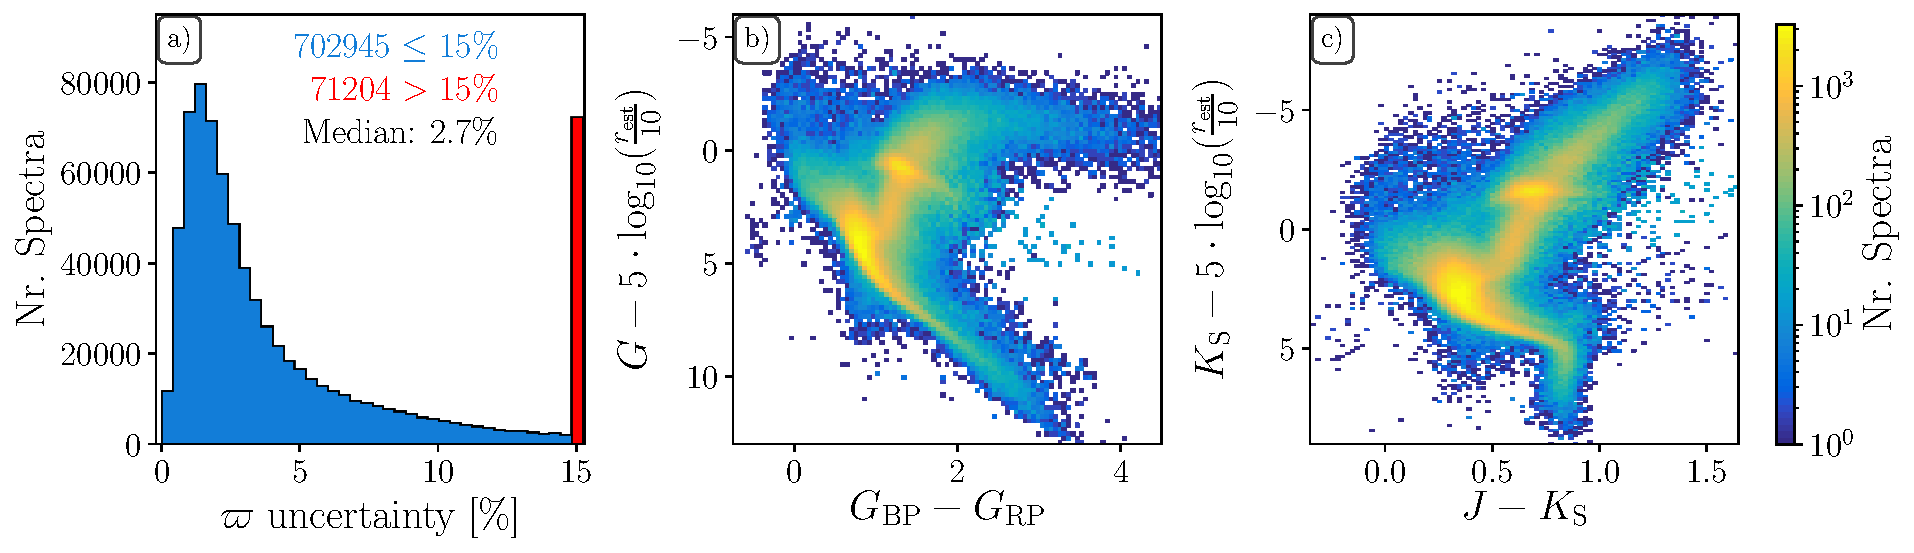
\includegraphics[width=\textwidth]{figures/plot_parallax_quality_and_cmds.pdf}
\caption{Overview of astro- and photometric information of the stars observed by GALAH until \SB{February 2019}. Panel a) shows the unprecedented parallax ($\varpi$) uncertainty provided by \Gaia DR2 with 702945 (91\%) spectra below 15\% (blue) and 71204 (9\%) spectra with uncertainties above 15\% (red, truncated). Panel b) shows a color-magnitude diagram as observed with the optical \Gaia passbands, whereas panel c) shows a color-magnitude diagram as observed with the infra-red 2MASS passbands. \SB{Note that not all of these stars are included in GALAH DR3}.}
\label{fig:plot_parallax_quality_and_cmds}
\end{figure*}

%________________________________________________________________
\section{Data analysis} \label{sec:analysis}

%________________________________________________________________
\subsection{Analysis flow and changes with respect to DR2} \label{sec:analysis_flow}

\begin{itemize}
\item SME only, no use of \textit{The Cannon} in this DR
\item Lay this out and motivate that by a figure, which shows 3 panels in the top for DR2 (Teff-logg, [Fe/H]-[alpha/Fe], [Fe/H]-A(Li)) and DR3 in the bottom
\item SME536, including changes as introduced by \citet{Piskunov2017}, but also with additional differences in the use of SME
\item using fundamental relation of surface gravity $\log g$ with available, non-spectroscopic information ($\varpi$ and $K_S$)
\item Workflow: 
\begin{enumerate}
	\item Estimate stellar parameters (\teff, \feh, \vbroad, \vrad from spectra, \logg via fundamental relation, \vmic via empirical relation)
	\item Validation of stellar parameters (see Sec.\ref{sec:validation_sp}), leading to an adjustment of the estimated atmospheric [Fe/H] (\textsc{sme.feh}) by adding $0.1\,\mathrm{dex}$\footnote{NB: This is not the final [Fe/H] as reported in this data release, but a pseudo iron abundance, estimated from H, Sc, Ti, and Fe lines.}
	\item Keep stellar parameters fixed and then estimate A(X) for element X. These can be done combined (write elements for which that was done) or on a line-by-line basis (write elements for which that was done).
\end{enumerate}
\end{itemize}

%________________________________________________________________
\subsection{Validation of stellar parameters} \label{sec:validation_sp}

To assess the quality of the stellar parameters, we resort to the commonly used comparison samples for accuracy, that is the GBS and the stars with asteroseismic information. For the precision assessment we use the internal uncertainty estimates and repeat observations of the same stars.  We calculate the final stellar parameter errors for a given parameter $X$ via 
\begin{equation}
e_\text{final}^2 (X) = e_\text{accuracy}^2(X) + e_\text{fit}^2(X) + e_\text{repeats}^2(X). \label{eq:final_error}
\end{equation}

We note that $e_\text{fit}^2(X)$ and $e_\text{repeats}^2(X)$ are typically expected to be the same tracer of precision and hence only their maximum value should be used, that is
\begin{equation}
e_\text{final}^2 (X) = e_\text{accuracy}^2(X) + \text{max} \left(e_\text{fit}^2(X) + e_\text{repeats}^2(X) \right).
\end{equation}

We elaborate on the choice of error combination when we assess the precision of the stellar parameters.

\subsubsection{Accuracy of stellar parameters}

\paragraph*{\Gaia FGK benchmark stars (GBS)}

\paragraph*{IRFM temperatures}

\paragraph*{Stars with asteroseismic information}

\subsubsection{Precision of stellar parameters}

- repeat observations and fitting uncertainties

\section{Validation of element abundances} \label{sec:validation_ab}

\subsubsection{Accuracy of element abundances}

\paragraph*{Abundances of the Sun}

\paragraph*{Abundances of Arcturus}

\paragraph*{Abundances of the GBS stars}

\paragraph*{TBD: Abundances of cluster stars?}

\subsubsection{Precision of element abundances}

\paragraph*{Abundances of repeat observations}

\paragraph*{TBD: Abundances of cluster stars?}

\subsection{The complexity and importance of flagging (and using them)}

\subsubsection{Flagging of stellar parameters}

\subsubsection{Flagging of element abundances}

We expect less trends without the influence of the training set selection or data-model flexibilities, but we still expect trends for several reasons:
\begin{itemize}
\item Given the model- and setup-imperfections, excluding \logg as a free fitting parameter might lead to systematic trends. This can be the case for those stars where the true \logg of the star and our estimated \logg differ significantly (e.g. binaries where the (unidentified) second component is contributing to the flux of the system) or the synthetic spectrum with the true \logg does not match the observation (e.g. due to shortcomings of the 1D model atmospheres and synthesis).
\item For stars with more lines, our pipeline will perform worse several ways. Firstly, estimating the continuum will be less reliable. Secondly, we will run into issues of strong blending, where our estimate is limited to how close the synthesis of the blending lines is to the true observation. If for example a star has scaled solar abundances, our estimates of the element abundances will still be good even for blended cases. If the compositions differs, and the line that we want to measure is blended by a line of a significantly over- or under-abundant element (relative to scaled-solar), our measurement might be corrupted. We try to limit this by performing a blending test, but setting the limit on how much blending is still acceptable is both non-trivial but also hard to flag during post-processing.
\item Due to time/computation restrictions, we were running several elements in a combined rather than line-by-line basis, which can decrease the precision as outlined in Sec.~\ref{sec:analysis_flow}, although we have tried to ensure that the abundance zero points of the individual lines were similar for those elements that were run with the combined setup.
\end{itemize}

\subsubsection{Expect the (un-)expected, but be cautious: Analysis shortcoming or physical correlation?}

\section{Catalogs included in this release}  \label{sec:catalogs}

%________________________________________________________________
\subsection{Main catalog} \label{sec:main_catalog}
\begin{enumerate}
\item Stellar paramaters (see Fig.~\ref{fig:hrd_galah_dr3})
\item Stellar parameter flags (both warning and flags)
\item Precision uncertainties and final uncertainties for each parameter (including accuracy, precision, and parameter node uncertainties)
\item Combined alpha-abundance (for unflagged measurements), see Fig.~\ref{fig:fe_h_alpha_fe}
\item Individual element abundances (including flagged measurements)
\item individual abundance flags
\item Precision uncertainties for each abundance
\item x-matches with Gaia DR2, Bailer-Jones2018, RUWE, 2MASS, WISE
\end{enumerate}

%________________________________________________________________
\subsection{Value-Added-Catalogs} \label{sec:value_added_catalogs}

The third Data Release of GALAH is accompanied by two value-added-catalogs and we explain them in this section. One value-added-catalog includes extended abundance measurement information, another one stellar ages as well as masses and a third one kinematic as well as dynamic information for each star.

\subsubsection{Extended abundance measurement information}

\subsubsection{Stellar age and mass estimates}

\subsubsection{Kinematic and dynamic information}

%________________________________________________________________
\section{GALAH DR3 in context} \label{sec:galah_in_context}

\subsection{Galactic archaeology on a global scale}  \label{sec:global_ga}

\subsection{Chemodynamical evolution}  \label{sec:cde}

Combining chemistry, dynamics, and ages of stars

- plot Galactic $v_R$ vs. $v_\phi$ (Belokurov)
- plot Toomre diagram
- plot actions
- plot \cite{Vasiliev2019} overview of $J_i$

%________________________________________________________________
\section{Conclusions} \label{sec:conclusions}


%________________________________________________________________
\section*{Acknowledgements}

Based on data acquired through the Australian Astronomical Observatory, under programmes: A/2013B/13 (The GALAH pilot survey); A/2014A/25, A/2015A/19, A2017A/18 (The GALAH survey phase 1), A2018 A/18 (Open clusters with HERMES), A2019A/1 (Hierarchical star formation in Ori OB1),  A2019A/15 (The GALAH survey phase 2), A/2015B/19, A/2016A/22, A/2016B/10, A/2017B/16, A/2018B/15 (The HERMES-TESS program), and A/2015A/3, A/2015B/1, A/2015B/19, A/2016A/22, A/2016B/12, A/2017A/14, (The HERMES K2-follow-up program). \SB{Are we missing programs?} We acknowledge the traditional owners of the land on which the AAT stands, the Gamilaraay people, and pay our respects to elders past and present.

This work has made use of data from the European Space Agency (ESA) mission \Gaia (http://www.cosmos.esa.int/gaia), processed by the \Gaia Data Processing and Analysis Consortium (DPAC, http://www.cosmos.esa.int/web/gaia/dpac/consortium). Funding for the DPAC has been provided by national institutions, in particular the institutions participating in the \Gaia Multilateral Agreement. 

The following software and programming languages made this research possible: \textsc{IRAF} \citep{Tody1986,Tody1993}, \textsc{configure} \citep{Miszalski2006}, \textsc{topcat} \citep[version 4.4;][]{Taylor2005}; Python (version 2.7) and its packages {\textsc{astropy}} \citep[version 2.0;][]{Robitaille2013,PriceWhelan2018}, {\textsc{matplotlib}} \citep{matplotlib}, {\textsc{pandas}} \citep[version 0.20.2;][]{McKinney2011}, {\textsc{NumPy}} \citep{numpy}, {\textsc{IPython}} \citep{ipython}, and  \textsc{galpy} \citep[version 1.3;][]{Bovy2015}. This research has made use of the VizieR catalogue access tool, CDS, Strasbourg, France. The original description of the VizieR service was published in A\&AS 143, 23. This research mad use of the TOPCAT tool, described in \citet{Taylor2005}. This publication makes use of data products from the Two Micron All Sky Survey, which is a joint project of the University of Massachusetts and the Infrared Processing and Analysis Center/California Institute of Technology, funded by the National Aeronautics and Space Administration and the National Science Foundation.

SB and acknowledges funds from the Alexander von Humboldt Foundation in the framework of the Sofja Kovalevskaja Award endowed by the Federal Ministry of Education and Research. SB acknowledges travel support from Universities Australia and Deutsche Akademische Austauschdienst.

%%%%%%%%%%%%%%%%%%%%%%%%%%%%%%%%%%%%%%%%%%%%%%%%%%

%%%%%%%%%%%%%%%%%%%% REFERENCES %%%%%%%%%%%%%%%%%%

% The best way to enter references is to use BibTeX:

\bibliographystyle{mnras}
\bibliography{bib} % if your bibtex file is called example.bib

%%%%%%%%%%%%%%%%%%%%%%%%%%%%%%%%%%%%%%%%%%%%%%%%%%

\newpage
\noindent \rule{8.5cm}{1pt}

\noindent
% List of institutions
$^{1}$Max Planck Institute  for Astronomy (MPIA), Koenigstuhl 17, 69117 Heidelberg, Germany\\
$^{2}$Research School of Astronomy \& Astrophysics, Australian National University, ACT 2611, Australia\\
$^{3}$Center of Excellence for Astrophysics in Three Dimensions (ASTRO-3D), Australia\\

%%%%%%%%%%%%%%%%% APPENDICES %%%%%%%%%%%%%%%%%%%%%

\appendix

\section{Linelist}\label{sec:linelist}

\begin{table*}
\caption{Selected lines for the elemental abundance analysis.}\label{linelist}
  \label{tab:linelist}
\centering
\begin{tabular}{l l l l l p{2.8cm} l l}
\hline
Elem. & Ion & Wavelength [\AA] & LEP [eV] & $\log(gf)$ & Reference & Line mask [\AA] & Segment mask [\AA] \\                                                                                            
\hline    
Li & 1 &6707.7635 & 0.00000 & -0.00200000 & 1998PhRvA..57.1652Y & 6707.3000-6708.3000 & 6705.76-6709.76 \\                                                                                              
Li & 1 &6707.9145 & 0.00000 & -0.303000 & 1998PhRvA..57.1652Y & 6707.3000-6708.3000 & 6705.76-6709.76 \\                                                                                                
Li & 1 &6707.9215 & 0.00000 & -0.00200000 & 1998PhRvA..57.1652Y & 6707.3000-6708.3000 & 6705.76-6709.76 \\                                                                                              
Li & 1 &6708.0725 & 0.00000 & -0.303000 & 1998PhRvA..57.1652Y & 6707.3000-6708.3000 & 6705.76-6709.76 \\                                                                                                
C  & 1 &6587.6100 & 8.53700 & -1.02100 & 1993A\&AS...99..179H & 6587.2610-6587.9860 & 6585.61-6589.61 \\                                                                                                
O  & 1 &7771.9440 & 9.14600 & 0.369000 & NIST & 7771.3590-7772.5090 & 7769.50-7777.50 \\                                                                                                                
O  & 1 &7774.1660 & 9.14600 & 0.223000 & NIST & 7773.5220-7774.7820 & 7769.50-7777.50 \\                                                                                                                
O  & 1 &7775.3880 & 9.14600 & 0.00200000 & NIST & 7774.9120-7775.9620 & 7769.50-7777.50 \\                                                                                                              
Na & 1 &5682.6333 & 2.10200 & -0.706000 & GESMCHF & 5682.5170-5682.9970 & 5680.63-5691.20 \\                                                                                                            
Na & 1 &5688.2050 & 2.10400 & -0.404000 & GESMCHF & 5687.9170-5688.3920 & 5680.63-5691.20 \\                                                                                                            
Mg & 1 &5711.0880 & 4.34600 & -1.72400 & 1990JQSRT..43..207C & 5710.7570-5711.4280 & 5710.00-5713.09 \\                                                                                                 
Al & 1 &6696.0230 & 3.14300 & -1.56900 & 2008JPCRD..37..709K & 6695.7780-6696.1730 & 6695.00-6699.87 \\                                                                                                 
Al & 1 &6698.6730 & 3.14300 & -1.87000 & 2008JPCRD..37..709K & 6698.3920-6698.8950 & 6695.00-6699.87 \\                                                                                                 
Al & 1 &7835.3090 & 4.02200 & -0.689000 & 2008JPCRD..37..709K & 7834.8840-7835.5720 & 7834.00-7837.50 \\                                                                                                
Al & 1 &7836.1340 & 4.02200 & -0.534000 & 2008JPCRD..37..709K & 7835.8130-7836.4310 & 7834.00-7837.50 \\                                                                                                
Al & 1 &7836.1340 & 4.02200 & -1.83400 & 2008JPCRD..37..709K & 7835.8130-7836.4310 & 7834.00-7837.50 \\                                                                                                 
Si & 1 &5684.4840 & 4.95400 & -1.55300 & GARZ|BL & 5684.1840-5684.7840 & 5683.00-5686.00 \\                                                                                                             
Si & 1 &5690.4250 & 4.93000 & -1.77300 & GARZ|BL & 5690.1800-5690.6830 & 5688.43-5692.43 \\                                                                                                             
Si & 1 &5701.1040 & 4.93000 & -1.95300 & GARZ|BL & 5700.9290-5701.2860 & 5699.70-5702.00 \\                                                                                                             
Si & 1 &5772.0272 & 5.61400 & -3.10700 & K07 & 5771.8460-5772.4460 & 5771.15-5773.15 \\                                                                                                                 
Si & 1 &5772.1460 & 5.08200 & -1.65300 & GARZ|BL & 5771.8460-5772.4460 & 5771.15-5773.15 \\                                                                                                             
Si & 1 &5793.0726 & 4.93000 & -1.96300 & GARZ|BL & 5792.7190-5793.3930 & 5791.07-5794.70 \\                                                                                                             
Si & 1 &6721.2732 & 5.96400 & -5.27200 & K07 & 6721.2000-6722.3000 & 6718.45-6723.85 \\                                                                                                                 
Si & 1 &6721.8481 & 5.86300 & -1.06200 & 1993PhyS...48..297N & 6721.2000-6722.3000 & 6718.45-6723.85 \\                                                                                                 
Si & 1 &7680.2660 & 5.86300 & -0.590000 & GARZ|BL & 7679.9440-7680.6680 & 7678.27-7682.27 \\                                                                                                            
K  & 1 &7698.9643 & 0.00000 & -0.178000 & 2017PhRvA..95e2507T & 7698.5730-7699.2960 & 7696.96-7700.96 \\                                                                                                

%Li & 1 &6707.7635 & 0.00000 & -0.00200000 & 1998PhRvA..57.1652Y & 6707.3000-6708.3000 & 6705.76-6709.76 \\                                                                                              
Li & 1 &6707.9145 & 0.00000 & -0.303000 & 1998PhRvA..57.1652Y & 6707.3000-6708.3000 & 6705.76-6709.76 \\                                                                                                
Li & 1 &6707.9215 & 0.00000 & -0.00200000 & 1998PhRvA..57.1652Y & 6707.3000-6708.3000 & 6705.76-6709.76 \\                                                                                              
Li & 1 &6708.0725 & 0.00000 & -0.303000 & 1998PhRvA..57.1652Y & 6707.3000-6708.3000 & 6705.76-6709.76 \\                                                                                                
C  & 1 &6587.6100 & 8.53700 & -1.02100 & 1993A\&AS...99..179H & 6587.2610-6587.9860 & 6585.61-6589.61 \\                                                                                                
O  & 1 &7771.9440 & 9.14600 & 0.369000 & NIST & 7771.3590-7772.5090 & 7769.50-7777.50 \\                                                                                                                
O  & 1 &7774.1660 & 9.14600 & 0.223000 & NIST & 7773.5220-7774.7820 & 7769.50-7777.50 \\                                                                                                                
O  & 1 &7775.3880 & 9.14600 & 0.00200000 & NIST & 7774.9120-7775.9620 & 7769.50-7777.50 \\                                                                                                              
Na & 1 &5682.6333 & 2.10200 & -0.706000 & GESMCHF & 5682.5170-5682.9970 & 5680.63-5691.20 \\                                                                                                            
Na & 1 &5688.2050 & 2.10400 & -0.404000 & GESMCHF & 5687.9170-5688.3920 & 5680.63-5691.20 \\                                                                                                            
Mg & 1 &5711.0880 & 4.34600 & -1.72400 & 1990JQSRT..43..207C & 5710.7570-5711.4280 & 5710.00-5713.09 \\                                                                                                 
Al & 1 &6696.0230 & 3.14300 & -1.56900 & 2008JPCRD..37..709K & 6695.7780-6696.1730 & 6695.00-6699.87 \\                                                                                                 
Al & 1 &6698.6730 & 3.14300 & -1.87000 & 2008JPCRD..37..709K & 6698.3920-6698.8950 & 6695.00-6699.87 \\                                                                                                 
Al & 1 &7835.3090 & 4.02200 & -0.689000 & 2008JPCRD..37..709K & 7834.8840-7835.5720 & 7834.00-7837.50 \\                                                                                                
Al & 1 &7836.1340 & 4.02200 & -0.534000 & 2008JPCRD..37..709K & 7835.8130-7836.4310 & 7834.00-7837.50 \\                                                                                                
Al & 1 &7836.1340 & 4.02200 & -1.83400 & 2008JPCRD..37..709K & 7835.8130-7836.4310 & 7834.00-7837.50 \\                                                                                                 
Si & 1 &5684.4840 & 4.95400 & -1.55300 & GARZ|BL & 5684.1840-5684.7840 & 5683.00-5686.00 \\                                                                                                             
Si & 1 &5690.4250 & 4.93000 & -1.77300 & GARZ|BL & 5690.1800-5690.6830 & 5688.43-5692.43 \\                                                                                                             
Si & 1 &5701.1040 & 4.93000 & -1.95300 & GARZ|BL & 5700.9290-5701.2860 & 5699.70-5702.00 \\                                                                                                             
Si & 1 &5772.0272 & 5.61400 & -3.10700 & K07 & 5771.8460-5772.4460 & 5771.15-5773.15 \\                                                                                                                 
Si & 1 &5772.1460 & 5.08200 & -1.65300 & GARZ|BL & 5771.8460-5772.4460 & 5771.15-5773.15 \\                                                                                                             
Si & 1 &5793.0726 & 4.93000 & -1.96300 & GARZ|BL & 5792.7190-5793.3930 & 5791.07-5794.70 \\                                                                                                             
Si & 1 &6721.2732 & 5.96400 & -5.27200 & K07 & 6721.2000-6722.3000 & 6718.45-6723.85 \\                                                                                                                 
Si & 1 &6721.8481 & 5.86300 & -1.06200 & 1993PhyS...48..297N & 6721.2000-6722.3000 & 6718.45-6723.85 \\                                                                                                 
Si & 1 &7680.2660 & 5.86300 & -0.590000 & GARZ|BL & 7679.9440-7680.6680 & 7678.27-7682.27 \\                                                                                                            
K  & 1 &7698.9643 & 0.00000 & -0.178000 & 2017PhRvA..95e2507T & 7698.5730-7699.2960 & 7696.96-7700.96 \\                                                                                                
Ca & 1 &5857.1962 & 5.30000 & -2.66500 & K07 & 5857.0180-5857.6250 & 5855.45-5859.45 \\                                                                                                                 
Ca & 1 &5857.4510 & 2.93300 & 0.240000 & S & 5857.0180-5857.6250 & 5855.45-5859.45 \\                                                                                                                   
Ca & 1 &5867.5620 & 2.93300 & -1.57000 & S & 5867.3000-5867.7000 & 5865.50-5869.80 \\                                                                                                                   
Ca & 1 &6493.7810 & 2.52100 & -0.109000 & SR & 6493.4650-6493.9930 & 6491.78-6501.65 \\                                                                                                                 
Ca & 1 &6493.8033 & 5.63200 & -4.55900 & K07 & 6493.4650-6493.9930 & 6491.78-6501.65 \\                                                                                                                 
Ca & 1 &6499.6500 & 2.52300 & -0.818000 & SR & 6499.3780-6499.9550 & 6491.78-6501.65 \\                                                                                                                 
Sc & 1 &4743.8300 & 1.44800 & 0.422000 & LD & 4743.5490-4744.0000 & 4741.83-4746.83 \\                                                                                                                  
Sc & 1 &4753.1610 & 0.00000 & -1.65900 & LD & 4753.0000-4753.4000 & 4751.30-4755.50 \\                                                                                                                  
Sc & 2 &5657.8960 & 1.50700 & -0.603000 & LD & 5657.6780-5658.1220 & 5655.90-5659.90 \\                                                                                                                 
Sc & 2 &5667.1490 & 1.50000 & -1.30900 & LD & 5666.9060-5667.3230 & 5665.15-5669.15 \\                                                                                                                  
Sc & 1 &5671.7751 & 1.44800 & -0.505000 & LD & 5671.6050-5672.0920 & 5669.82-5673.82 \\                                                                                                                 
Sc & 1 &5671.7898 & 1.44800 & -0.209000 & LD & 5671.6050-5672.0920 & 5669.82-5673.82 \\                                                                                                                 
Sc & 1 &5671.8032 & 1.44800 & -0.471000 & LD & 5671.6050-5672.0920 & 5669.82-5673.82 \\                                                                                                                 
Sc & 1 &5671.8163 & 1.44800 & -0.290000 & LD & 5671.6050-5672.0920 & 5669.82-5673.82 \\                                                                                                                 
Sc & 1 &5671.8271 & 1.44800 & -1.02700 & LD & 5671.6050-5672.0920 & 5669.82-5673.82 \\                                                                                                                  
Sc & 1 &5671.8436 & 1.44800 & -0.232000 & LD & 5671.6050-5672.0920 & 5669.82-5673.82 \\                                                                                                                 
Sc & 1 &5671.8641 & 1.44800 & -0.178000 & LD & 5671.6050-5672.0920 & 5669.82-5673.82 \\                                                                                                                 
Sc & 1 &5717.3070 & 1.44000 & -0.532000 & LD & 5717.0000-5717.5000 & 5715.50-5719.50 \\                                                                                                                 
Sc & 1 &5724.1070 & 1.43300 & -0.661000 & LD & 5723.8940-5724.2690 & 5722.11-5726.11 \\                                                                                                                 
Sc & 2 &6604.6010 & 1.35700 & -1.30900 & LD & 6604.4090-6604.9790 & 6602.60-6606.60 \\                                                                                                                  
Ti & 1 &4758.1178 & 2.24900 & 0.510000 & LGWSC & 4757.9470-4758.3060 & 4756.12-4760.12 \\                                                                                                               
Ti & 1 &4759.1416 & 2.77800 & -3.00200 & K10 & 4759.0880-4759.4910 & 4756.12-4760.12 \\                                                                                                                 
Ti & 1 &4759.2697 & 2.25600 & 0.590000 & LGWSC & 4759.0880-4759.4910 & 4756.12-4760.12 \\                                                                                                               
Ti & 1 &4778.2547 & 2.23600 & -0.350000 & LGWSC & 4778.0790-4778.4420 & 4776.25-4780.00 \\                                                                                                              
Ti & 1 &4781.7106 & 0.848000 & -1.95000 & LGWSC & 4781.5730-4781.9310 & 4780.50-4782.76 \\                                                                                                              
Ti & 1 &4797.9757 & 2.33400 & -0.630000 & LGWSC & 4797.8350-4798.1290 & 4796.33-4799.41 \\                                                                                                              
Ti & 1 &4801.9016 & 0.818000 & -3.06000 & LGWSC & 4801.8000-4802.2000 & 4800.00-4803.90 \\                                                                                                              
Ti & 1 &4801.9486 & 0.826000 & -3.16000 & LGWSC & 4801.8000-4802.2000 & 4800.00-4803.90 \\                                                                                                              
Ti & 1 &4802.1370 & 2.24900 & -3.84500 & K10 & 4801.8000-4802.2000 & 4800.00-4803.90 \\                                                                                                                 
Ti & 1 &4820.2488 & 3.70900 & -5.44900 & K10 & 4820.0880-4820.6700 & 4818.41-4822.41 \\                                                                                                                 
Ti & 2 &4820.3706 & 5.90500 & -2.03700 & K10 & 4820.0880-4820.6700 & 4818.41-4822.41 \\                                                                                                                 
Ti & 1 &4820.4094 & 1.50300 & -0.380000 & LGWSC & 4820.0880-4820.6700 & 4818.41-4822.41 \\                                                                                                              
Ti & 1 &5689.4600 & 2.29700 & -0.360000 & NWL & 5689.2640-5689.8050 & 5687.46-5691.46 \\                                                                                                                
Ti & 1 &5716.4500 & 2.29700 & -0.720000 & NWL & 5716.2320-5716.8300 & 5714.45-5718.45 \\                                                                                                                
Ti & 1 &5716.7175 & 3.42400 & -3.00600 & K10 & 5716.2320-5716.8300 & 5714.45-5718.45 \\                                                                                                                 
Ti & 1 &5720.4359 & 2.29200 & -0.900000 & MFW & 5720.2450-5720.6750 & 5718.50-5722.50 \\                                                                                                                
Ti & 1 &5720.6453 & 3.29400 & -2.80700 & K10 & 5720.2450-5720.6750 & 5718.50-5722.50 \\                                                                                                                 
Ti & 1 &5739.4690 & 2.24900 & -0.610000 & LGWSC & 5739.2500-5739.7000 & 5737.47-5741.47 \\                                                                                                              
Ti & 1 &5866.3679 & 3.30500 & -1.05500 & K10 & 5866.0000-5866.8090 & 5864.79-5868.60 \\                                                                                                                 
Ti & 1 &5866.4513 & 1.06700 & -0.790000 & LGWSC & 5866.0000-5866.8090 & 5864.79-5868.60 \\                                                                                                              
Ti & 2 &5866.6643 & 8.08900 & -0.695000 & K10 & 5866.0000-5866.8090 & 5864.79-5868.60 \\                                                                                                                
Ti & 1 &5866.8072 & 3.32300 & -2.21300 & K10 & 5866.0000-5866.8090 & 5864.79-5868.60 \\                                                                                                                 
Ti & 1 &6599.1048 & 0.900000 & -2.02900 & 1983MNRAS.204..883B|1989A\&A...208..157G & 6598.8980-6599.4980 & 6597.11-6601.11 \\                                                                           
Ti & 1 &6716.6660 & 2.48800 & -1.37000 & LGWSC & 6716.4890-6716.9050 & 6714.67-6718.67 \\                                                                                                               
Ti & 1 &7852.6770 & 0.848000 & -2.64000 & BLNP & 7852.2000-7852.9970 & 7851.36-7854.67 \\                                                                                                               
Ti & 1 &7852.6819 & 1.87900 & -4.09600 & K10 & 7852.2000-7852.9970 & 7851.36-7854.67 \\                                                                                                                 
Ti & 1 &4719.3556 & 0.813000 & -4.45900 & K10 & 4719.3000-4719.6000 & 4719.00-4721.51 \\                                                                                                                
Ti & 2 &4719.5109 & 1.24300 & -3.32000 & WLSC & 4719.3000-4719.6000 & 4719.00-4721.51 \\                                                                                                                
Ti & 2 &4764.5247 & 1.23700 & -2.69000 & WLSC & 4764.3970-4764.8000 & 4762.52-4766.52 \\                                                                                                                
Ti & 2 &4798.5313 & 1.08000 & -2.66000 & WLSC & 4798.3300-4798.6440 & 4796.33-4799.41 \\                                                                                                                
Ti & 2 &4849.1678 & 1.13100 & -2.96000 & WLSC & 4849.0500-4849.4000 & 4847.17-4851.17 \\                                                                                                                
Ti & 2 &4865.6104 & 1.11600 & -2.70000 & WLSC & 4865.3000-4865.8500 & 4863.61-4867.61 \\                                                                                                                
Ti & 1 &4865.7808 & 2.57800 & -2.00000 & MA-astro & 4865.3000-4865.8500 & 4863.61-4867.61 \\                                                                                                            
Ti & 2 &4874.0094 & 3.09500 & -0.860000 & WLSC & 4873.8700-4874.1940 & 4872.01-4876.01 \\                                                                                                               
V  & 1 &4831.6457 & 0.0170000 & -1.38000 & 2014ApJS..215...20L & 4831.5250-4831.7290 & 4829.65-4833.65 \\                                                                                               
V  & 1 &4784.4665 & 0.0170000 & -2.67000 & 2014ApJS..215...20L & 4784.3360-4784.6070 & 4782.47-4786.47 \\                                                                                               
V  & 1 &4796.9140 & 2.09700 & 0.190000 & 2014ApJS..215...20L & 4796.7600-4796.9750 & 4794.91-4798.91 \\                                                                                                 
Cr & 1 &4775.1300 & 3.55100 & -1.05000 & MFW & 4774.9500-4775.3070 & 4773.13-4777.13 \\                                                                                                                 
Cr & 1 &4789.3350 & 2.54400 & -0.330000 & SLS & 4789.1930-4789.4820 & 4787.33-4791.33 \\                                                                                                                
Cr & 1 &4801.0247 & 3.12200 & -0.131000 & MFW & 4800.8390-4801.2330 & 4799.02-4803.02 \\                                                                                                                
Cr & 1 &5787.9190 & 3.32200 & -0.0830000 & MFW & 5787.6400-5788.1600 & 5786.32-5790.42 \\                                                                                                               
Cr & 1 &6630.0100 & 1.03000 & -3.56000 & MFW & 6629.7740-6630.2720 & 6627.51-6632.51 \\                                                                                                                 
Mn & 1 &4738.9176 & 3.77200 & -3.89500 & K07 & 4738.8970-4739.3040 & 4737.09-4741.09 \\                                                                                                                 
Mn & 1 &4739.0900 & 2.94100 & -0.604000 & DLSSC & 4738.8970-4739.3040 & 4737.09-4741.09 \\                                                                                                              
Mn & 1 &4753.8969 & 5.21400 & -0.920000 & K07 & 4753.8000-4754.3000 & 4752.04-4755.60 \\                                                                                                                
Mn & 1 &4754.0183 & 2.28200 & -0.647000 & DLSSC & 4753.8000-4754.3000 & 4752.04-4755.60 \\                                                                                                              
Mn & 1 &4754.0301 & 2.28200 & -0.787000 & DLSSC & 4753.8000-4754.3000 & 4752.04-4755.60 \\                                                                                                              
Mn & 1 &4754.0472 & 2.28200 & -0.668000 & DLSSC & 4753.8000-4754.3000 & 4752.04-4755.60 \\                                                                                                              
Mn & 2 &4754.0558 & 6.13900 & -3.12400 & K09 & 4753.8000-4754.3000 & 4752.04-4755.60 \\                                                                                                                 
Mn & 1 &4754.0635 & 2.28200 & -0.670000 & DLSSC & 4753.8000-4754.3000 & 4752.04-4755.60 \\                                                                                                              
Mn & 1 &4754.0784 & 2.28200 & -1.84000 & DLSSC & 4753.8000-4754.3000 & 4752.04-4755.60 \\                                                                                                               
Mn & 1 &4761.4912 & 2.95300 & -1.16600 & DLSSC & 4761.3520-4761.7620 & 4759.51-4763.51 \\                                                                                                               
Mn & 1 &4761.5060 & 2.95300 & -0.548000 & DLSSC & 4761.3520-4761.7620 & 4759.51-4763.51 \\                                                                                                              
Mn & 1 &4761.5198 & 2.95300 & -0.821000 & DLSSC & 4761.3520-4761.7620 & 4759.51-4763.51 \\                                                                                                              
Mn & 1 &4761.5408 & 2.95300 & -1.61300 & DLSSC & 4761.3520-4761.7620 & 4759.51-4763.51 \\                                                                                                               
Mn & 1 &4765.8380 & 2.94100 & -0.601000 & DLSSC & 4765.7110-4766.0570 & 4763.85-4767.85 \\                                                                                                              
Mn & 1 &4765.8525 & 2.94100 & -0.445000 & DLSSC & 4765.7110-4766.0570 & 4763.85-4767.85 \\                                                                                                              
Mn & 1 &4765.8647 & 2.94100 & -0.676000 & DLSSC & 4765.7110-4766.0570 & 4763.85-4767.85 \\                                                                                                              
Mn & 1 &4766.0086 & 4.42500 & -3.05400 & K07 & 4765.7110-4766.0570 & 4763.85-4767.85 \\                                                                                                                 
Fe & 1 &4788.7566 & 3.23700 & -1.76300 & BWL & 4788.5550-4788.9960 & 4787.50-4790.00 \\                                                                                                                 
Fe & 1 &4788.7786 & 4.14300 & -2.52300 & K14 & 4788.5550-4788.9960 & 4787.50-4790.00 \\                                                                                                                 
Fe & 1 &4793.9614 & 3.04700 & -3.43000 & MRW & 4793.8310-4794.1490 & 4792.80-4795.50 \\                                                                                                                 
Fe & 1 &4794.3541 & 2.42400 & -3.95000 & MRW & 4794.2370-4794.5460 & 4792.80-4795.50 \\                                                                                                                 
Fe & 1 &4802.8746 & 3.69500 & -2.02800 & K14 & 4802.6740-4803.0860 & 4801.70-4804.10 \\                                                                                                                 
Fe & 1 &4802.8797 & 3.64200 & -1.51000 & BWL & 4802.6740-4803.0860 & 4801.70-4804.10 \\                                                                                                                 
Fe & 1 &4803.0294 & 5.06400 & -2.94700 & K07 & 4802.6740-4803.0860 & 4801.70-4804.10 \\                                                                                                                 
Fe & 1 &4808.1478 & 3.25100 & -2.69000 & MRW & 4807.9950-4808.3280 & 4807.00-4809.30 \\                                                                                                                 
Fe & 1 &4875.8770 & 3.33200 & -1.90000 & 2014MNRAS.441.3127R & 4875.7500-4876.1000 & 4874.75-4877.10 \\                                                                                                 
Fe & 2 &4889.6227 & 0.0480000 & -8.09900 & K13 & 4889.5000-4890.9990 & 4888.50-4893.50 \\                                                                                                               
Fe & 2 &4889.6848 & 7.98800 & -3.75500 & RU & 4889.5000-4890.9990 & 4888.50-4893.50 \\                                                                                                                  
Fe & 2 &4889.7133 & 0.107000 & -14.0240 & K13 & 4889.5000-4890.9990 & 4888.50-4893.50 \\                                                                                                                
Fe & 2 &4889.7133 & 0.107000 & -12.1940 & K13 & 4889.5000-4890.9990 & 4888.50-4893.50 \\                                                                                                                
Fe & 1 &4889.7740 & 3.63400 & -9.84800 & K14 & 4889.5000-4890.9990 & 4888.50-4893.50 \\                                                                                                                 
Fe & 1 &4890.5192 & 4.30100 & -3.84600 & K14 & 4889.5000-4890.9990 & 4888.50-4893.50 \\                                                                                                                 
Fe & 1 &4890.7551 & 2.87600 & -0.386000 & BWL+2014MNRAS.441.3127R & 4889.5000-4890.9990 & 4888.50-4893.50 \\                                                                                            
Fe & 1 &4890.8477 & 4.54900 & -5.09400 & K14 & 4889.5000-4890.9990 & 4888.50-4893.50 \\                                                                                                                 
Fe & 1 &4890.9101 & 4.22000 & -2.45000 & K14 & 4889.5000-4890.9990 & 4888.50-4893.50 \\                                                                                                                 
Fe & 1 &4890.9620 & 4.58400 & -4.91200 & K14 & 4889.5000-4890.9990 & 4888.50-4893.50 \\                                                                                                                 
Fe & 1 &4891.4921 & 2.85100 & -0.111000 & BWL & 4891.2570-4892.5000 & 4888.50-4893.50 \\                                                                                                                
Fe & 1 &4891.7573 & 4.47300 & -5.09500 & K14 & 4891.2570-4892.5000 & 4888.50-4893.50 \\                                                                                                                 
Fe & 2 &4892.2622 & 6.70300 & -3.06800 & RU & 4891.2570-4892.5000 & 4888.50-4893.50 \\                                                                                                                  
Fe & 1 &5651.4689 & 4.47300 & -1.90000 & MRW & 5651.3150-5651.6460 & 5650.30-5653.50 \\                                                                                                                 
Fe & 2 &5651.5235 & 10.6290 & -0.615000 & RU & 5651.3150-5651.6460 & 5650.30-5653.50 \\                                                                                                                 
Fe & 1 &5651.5251 & 4.44600 & -4.76100 & K07 & 5651.3150-5651.6460 & 5650.30-5653.50 \\                                                                                                                 
Fe & 2 &5651.6338 & 10.6290 & -1.01000 & RU & 5651.3150-5651.6460 & 5650.30-5653.50 \\                                                                                                                  
Fe & 1 &5652.3176 & 4.26000 & -1.85000 & MRW & 5652.1100-5652.5330 & 5650.30-5653.50 \\                                                                                                                 
Fe & 1 &5661.2361 & 4.79500 & -3.94200 & K14 & 5661.1640-5661.6530 & 5660.20-5663.70 \\                                                                                                                 
Fe & 1 &5661.2813 & 4.19100 & -3.50100 & K14 & 5661.1640-5661.6530 & 5660.20-5663.70 \\                                                                                                                 
Fe & 1 &5661.3447 & 4.28400 & -1.75600 & BK & 5661.1640-5661.6530 & 5660.20-5663.70 \\                                                                                                                  
Fe & 1 &5662.5161 & 4.17800 & -0.447000 & BWL+GESHRL14 & 5662.3000-5662.7000 & 5660.20-5663.70 \\                                                                                                       
Fe & 1 &5679.0229 & 4.65200 & -0.820000 & MRW & 5678.8100-5679.3480 & 5677.80-5681.50 \\                                                                                                                
Fe & 1 &5679.0351 & 5.34100 & -6.57900 & K07 & 5678.8100-5679.3480 & 5677.80-5681.50 \\                                                                                                                 
Fe & 1 &5679.1187 & 5.03300 & -1.98400 & K14 & 5678.8100-5679.3480 & 5677.80-5681.50 \\                                                                                                                 
Fe & 2 &5680.1971 & 3.38700 & -10.1260 & K13 & 5680.0760-5680.4730 & 5677.80-5681.50 \\                                                                                                                 
Fe & 2 &5680.1971 & 3.38700 & -9.20800 & K13 & 5680.0760-5680.4730 & 5677.80-5681.50 \\                                                                                                                 
Fe & 1 &5680.2404 & 4.18600 & -2.48000 & MRW & 5680.0760-5680.4730 & 5677.80-5681.50 \\                                                                                                                 
Fe & 1 &5696.0892 & 4.54900 & -1.72000 & BK & 5695.9420-5696.2230 & 5694.10-5697.20 \\                                                                                                                  
Fe & 2 &5696.1099 & 2.64200 & -8.10300 & K13 & 5695.9420-5696.2230 & 5694.10-5697.20 \\                                                                                                                 
Fe & 1 &5701.4161 & 3.21100 & -3.84800 & K14 & 5701.3500-5701.8000 & 5700.35-5702.80 \\                                                                                                                 
Fe & 1 &5701.5136 & 4.91300 & -1.25100 & K14 & 5701.3500-5701.8000 & 5700.35-5702.80 \\                                                                                                                 
Fe & 1 &5701.5442 & 2.55900 & -2.19300 & BK+GESB82d+BWL & 5701.3500-5701.8000 & 5700.35-5702.80 \\                                                                                                      
Fe & 1 &5705.2799 & 4.98800 & -2.79200 & K14 & 5705.2070-5705.7030 & 5704.20-5706.70 \\                                                                                                                 
Fe & 1 &5705.3275 & 4.21800 & -4.12700 & K14 & 5705.2070-5705.7030 & 5704.20-5706.70 \\                                                                                                                 
Fe & 1 &5705.4642 & 4.30100 & -1.35500 & BK & 5705.2070-5705.7030 & 5704.20-5706.70 \\                                                                                                                  
Fe & 1 &5731.7618 & 4.25600 & -1.20000 & MRW & 5731.5000-5732.0830 & 5730.10-5733.50 \\                                                                                                                 
Fe & 1 &5732.2960 & 4.99100 & -1.46000 & MRW & 5732.0890-5732.4830 & 5730.10-5733.50 \\                                                                                                                 
Fe & 1 &5741.8477 & 4.25600 & -1.67200 & BWL & 5741.5080-5742.0070 & 5740.40-5744.30 \\                                                                                                                 
Fe & 2 &5741.9225 & 9.13000 & -3.30300 & RU & 5741.5080-5742.0070 & 5740.40-5744.30 \\                                                                                                                  
Fe & 1 &5774.9157 & 4.59300 & -3.38500 & K14 & 5774.8150-5775.4030 & 5773.02-5777.30 \\                                                                                                                 
Fe & 1 &5775.0541 & 0.0520000 & -10.1110 & K07 & 5774.8150-5775.4030 & 5773.02-5777.30 \\                                                                                                               
Fe & 1 &5775.0805 & 4.22000 & -1.08000 & 2014ApJS..215...23D & 5774.8150-5775.4030 & 5773.02-5777.30 \\                                                                                                 
Fe & 2 &5775.1712 & 6.80700 & -4.13400 & RU & 5774.8150-5775.4030 & 5773.02-5777.30 \\                                                                                                                  
Fe & 2 &5778.3521 & 1.07600 & -10.7520 & K13 & 5778.2000-5778.7000 & 5777.30-5779.30 \\                                                                                                                 
Fe & 1 &5778.4526 & 4.15400 & -4.36300 & K14 & 5778.2000-5778.7000 & 5777.30-5779.30 \\                                                                                                                 
Fe & 1 &5778.4533 & 2.58800 & -3.43000 & BK & 5778.2000-5778.7000 & 5777.30-5779.30 \\                                                                                                                  
Fe & 1 &5806.6270 & 4.91300 & -2.12100 & K14 & 5806.5000-5806.9000 & 5805.50-5808.00 \\                                                                                                                 
Fe & 1 &5806.7249 & 4.60800 & -0.950000 & MRW & 5806.5000-5806.9000 & 5805.50-5808.00 \\                                                                                                                
Fe & 2 &5806.8216 & 10.6780 & -1.32400 & RU & 5806.5000-5806.9000 & 5805.50-5808.00 \\                                                                                                                  
Fe & 1 &5809.1556 & 3.69500 & -3.13500 & K14 & 5809.0000-5809.5000 & 5808.00-5810.50 \\                                                                                                                 
Fe & 1 &5809.2174 & 3.88400 & -1.74000 & MRW & 5809.0000-5809.5000 & 5808.00-5810.50 \\                                                                                                                 
Fe & 2 &5809.4277 & 1.09700 & -10.9890 & K13 & 5809.0000-5809.5000 & 5808.00-5810.50 \\                                                                                                                 
Fe & 1 &5811.9144 & 4.14300 & -2.33000 & MRW & 5811.8000-5812.2000 & 5810.80-5813.20 \\                                                                                                                 
Fe & 2 &5811.9462 & 2.70400 & -5.91300 & RU & 5811.8000-5812.2000 & 5810.80-5813.20 \\                                                                                                                  
Fe & 1 &5814.8071 & 4.28300 & -1.87000 & MRW & 5814.7000-5815.0000 & 5813.70-5816.00 \\                                                                                                                 
Fe & 1 &5849.4649 & 5.35200 & -6.70200 & K07 & 5849.4630-5849.8590 & 5848.40-5850.85 \\                                                                                                                 
Fe & 1 &5849.5659 & 4.65200 & -7.23400 & K14 & 5849.4630-5849.8590 & 5848.40-5850.85 \\                                                                                                                 
Fe & 1 &5849.6323 & 3.63500 & -4.90500 & K14 & 5849.4630-5849.8590 & 5848.40-5850.85 \\                                                                                                                 
Fe & 1 &5849.6833 & 3.69500 & -2.89000 & MRW & 5849.4630-5849.8590 & 5848.40-5850.85 \\                                                                                                                 
Fe & 1 &5853.1483 & 1.48500 & -5.18000 & MRW & 5852.8540-5853.3090 & 5852.00-5854.00 \\                                                                                                                 
Fe & 1 &5855.0758 & 4.60800 & -1.47800 & BK & 5854.8020-5855.3230 & 5854.00-5856.30 \\                                                                                                                  
Fe & 1 &5858.6234 & 4.58000 & -5.96200 & K14 & 5858.5920-5859.0340 & 5857.50-5860.50 \\                                                                                                                 
Fe & 1 &5858.6642 & 4.55900 & -3.97200 & K14 & 5858.5920-5859.0340 & 5857.50-5860.50 \\                                                                                                                 
Fe & 1 &5858.7780 & 4.22000 & -2.16000 & MRW & 5858.5920-5859.0340 & 5857.50-5860.50 \\                                                                                                                 
Fe & 1 &5858.9784 & 2.46900 & -8.50300 & K14 & 5858.5920-5859.0340 & 5857.50-5860.50 \\                                                                                                                 
Fe & 1 &6475.6239 & 2.55900 & -2.94100 & BWL & 6475.2000-6475.9500 & 6474.00-6477.00 \\                                                                                                                 
Fe & 1 &6481.7248 & 3.57300 & -5.21200 & K14 & 6481.5910-6482.0760 & 6480.50-6483.40 \\                                                                                                                 
Fe & 1 &6481.8530 & 5.31400 & -4.18800 & K14 & 6481.5910-6482.0760 & 6480.50-6483.40 \\                                                                                                                 
Fe & 1 &6481.8698 & 2.27900 & -2.98100 & BKK+GESB82c+BWL & 6481.5910-6482.0760 & 6480.50-6483.40 \\                                                                                                     
Fe & 1 &6494.9804 & 2.40400 & -1.26800 & GESB82c+BWL & 6494.7500-6495.3000 & 6493.75-6496.30 \\                                                                                                         
Fe & 2 &6495.2099 & 11.0930 & 0.0310000 & K13 & 6494.7500-6495.3000 & 6493.75-6496.30 \\                                                                                                                
Fe & 1 &6498.7529 & 5.34500 & -4.51200 & K14 & 6498.5000-6499.3000 & 6497.50-6500.50 \\                                                                                                                 
Fe & 1 &6498.9383 & 0.958000 & -4.68700 & GESB86+BWL & 6498.5000-6499.3000 & 6497.50-6500.50 \\                                                                                                         
Fe & 1 &6499.0241 & 5.34800 & -6.94200 & K14 & 6498.5000-6499.3000 & 6497.50-6500.50 \\                                                                                                                 
Fe & 1 &6499.1838 & 4.47300 & -5.98800 & K14 & 6498.5000-6499.3000 & 6497.50-6500.50 \\                                                                                                                 
Fe & 1 &6518.3657 & 2.83200 & -2.43800 & BK+BWL & 6518.0000-6518.5780 & 6517.00-6519.50 \\                                                                                                              
Fe & 1 &6518.5171 & 5.47800 & -6.66700 & K07 & 6518.0000-6518.5780 & 6517.00-6519.50 \\                                                                                                                 
Fe & 1 &6545.9929 & 5.31400 & -3.53400 & K14 & 6545.8950-6546.6700 & 6544.90-6547.67 \\                                                                                                                 
Fe & 1 &6546.2381 & 2.75900 & -1.53600 & BWL & 6545.8950-6546.6700 & 6544.90-6547.67 \\                                                                                                                 
Fe & 1 &6592.9124 & 2.72800 & -1.47300 & BWL & 6592.6880-6593.4500 & 6591.70-6594.45 \\                                                                                                                 
Fe & 1 &6593.4094 & 5.39300 & -4.59900 & K14 & 6592.6880-6593.4500 & 6591.70-6594.45 \\                                                                                                                 
Fe & 1 &6593.8695 & 2.43300 & -2.42000 & BIPS & 6593.5000-6594.2700 & 6591.70-6594.45 \\                                                                                                                
Fe & 1 &6597.3577 & 5.35700 & -3.80600 & K14 & 6597.2350-6597.8650 & 6596.20-6598.80 \\                                                                                                                 
Fe & 2 &6597.4691 & 7.97000 & -3.05200 & RU & 6597.2350-6597.8650 & 6596.20-6598.80 \\                                                                                                                  
Fe & 1 &6597.5592 & 4.79500 & -0.970000 & MRW & 6597.2350-6597.8650 & 6596.20-6598.80 \\                                                                                                                
Fe & 1 &6608.7934 & 5.33000 & -4.56300 & K14 & 6608.6010-6609.4160 & 6607.60-6610.40 \\                                                                                                                 
Fe & 1 &6608.9516 & 4.19100 & -2.66000 & K14 & 6608.6010-6609.4160 & 6607.60-6610.40 \\                                                                                                                 
Fe & 1 &6609.1097 & 2.55900 & -2.69100 & BIPS & 6608.6010-6609.4160 & 6607.60-6610.40 \\                                                                                                                
Fe & 2 &6609.2351 & 7.12800 & -2.87300 & RU & 6608.6010-6609.4160 & 6607.60-6610.40 \\                                                                                                                  
Fe & 1 &6627.5438 & 4.54900 & -1.59000 & 2014MNRAS.441.3127R & 6627.3460-6627.8490 & 6626.50-6628.80 \\                                                                                                 
Fe & 1 &6648.0796 & 1.01100 & -5.91800 & GESB86 & 6647.8000-6648.4000 & 6646.80-6649.40 \\                                                                                                              
Fe & 1 &6677.7219 & 5.47800 & -2.46300 & K14 & 6677.7000-6678.3000 & 6676.70-6679.30 \\                                                                                                                 
Fe & 1 &6677.7701 & 4.83500 & -1.81900 & K07 & 6677.7000-6678.3000 & 6676.70-6679.30 \\                                                                                                                 
Fe & 1 &6677.9534 & 2.55900 & -3.67100 & K14 & 6677.7000-6678.3000 & 6676.70-6679.30 \\                                                                                                                 
Fe & 1 &6677.9851 & 2.69200 & -1.41800 & BWL & 6677.7000-6678.3000 & 6676.70-6679.30 \\                                                                                                                 
Fe & 1 &6699.1413 & 4.59300 & -2.10100 & BKK & 6698.9260-6699.4370 & 6697.90-6700.50 \\                                                                                                                 
Fe & 2 &6699.1682 & 5.95600 & -4.06000 & RU & 6698.9260-6699.4370 & 6697.90-6700.50 \\                                                                                                                  
Fe & 1 &6699.3186 & 4.41500 & -4.31500 & K14 & 6698.9260-6699.4370 & 6697.90-6700.50 \\                                                                                                                 
Fe & 1 &6703.4199 & 3.64200 & -4.08400 & K14 & 6703.1840-6703.7970 & 6702.20-6704.80 \\                                                                                                                 
Fe & 1 &6703.5660 & 2.75900 & -3.06000 & MRW & 6703.1840-6703.7970 & 6702.20-6704.80 \\                                                                                                                 
Fe & 1 &6713.5207 & 5.58700 & -2.99800 & K07 & 6713.5000-6714.1450 & 6712.50-6715.20 \\                                                                                                                 
Fe & 1 &6713.7425 & 4.79500 & -1.50000 & MRW & 6713.5000-6714.1450 & 6712.50-6715.20 \\                                                                                                                 
Fe & 1 &6714.0955 & 5.48600 & -3.73900 & K07 & 6713.5000-6714.1450 & 6712.50-6715.20 \\                                                                                                                 
Fe & 1 &6725.3558 & 4.10300 & -2.10000 & 2014MNRAS.441.3127R & 6725.0000-6725.6000 & 6724.00-6726.60 \\                                                                                                 
Fe & 1 &6725.4354 & 5.60700 & -2.02600 & K07 & 6725.0000-6725.6000 & 6724.00-6726.60 \\                                                                                                                 
Fe & 1 &6732.8102 & 2.45300 & -10.3400 & K07 & 6732.8000-6733.4000 & 6731.80-6734.40 \\                                                                                                                 
Fe & 1 &6733.1503 & 4.63800 & -1.48000 & MRW & 6732.8000-6733.4000 & 6731.80-6734.40 \\                                                                                                                 
Fe & 1 &6739.5204 & 1.55700 & -4.79400 & BKK & 6739.2000-6739.8000 & 6738.00-6741.00 \\                                                                                                                 
Fe & 2 &4720.1263 & 9.74200 & -3.06800 & RU & 4720.0010-4720.2800 & 4719.00-4721.00 \\                                                                                                                  
Fe & 2 &4720.1386 & 3.19700 & -4.48000 & 2009A\&A...497..611M:solar-gf & 4720.0010-4720.2800 & 4719.00-4721.00 \\                                                                                       
Fe & 2 &4731.4476 & 2.89100 & -3.10000 & 2009A\&A...497..611M & 4731.3050-4731.6600 & 4730.30-4732.60 \\                                                                                                
Fe & 1 &4731.5999 & 3.68600 & -2.60000 & KL-astro & 4731.3050-4731.6600 & 4730.30-4732.60 \\                                                                                                            
Fe & 2 &4833.1916 & 2.65700 & -4.64000 & 2009A\&A...497..611M:solar-gf & 4833.0000-4833.2650 & 4832.00-4834.30 \\                                                                                       
Fe & 2 &6516.0766 & 2.89100 & -3.31000 & 2009A\&A...497..611M & 6515.8330-6516.4120 & 6514.80-6517.00 \\                                                                                                
Fe & 1 &7711.4200 & 5.53900 & -5.82200 & K07 & 7711.2520-7712.1600 & 7709.00-7713.20 \\                                                                                                                 
Fe & 2 &7711.4385 & 5.51100 & -2.90400 & RU & 7711.2520-7712.1600 & 7709.00-7713.20 \\                                                                                                                  
Fe & 1 &7711.5497 & 5.53900 & -4.74600 & K14 & 7711.2520-7712.1600 & 7709.00-7713.20 \\                                                                                                                 
Fe & 2 &7711.7204 & 3.90300 & -2.50000 & 2009A\&A...497..611M & 7711.2520-7712.1600 & 7709.00-7713.20 \\                                                                                                
Co & 1 &4781.4283 & 1.88300 & -2.15000 & FMW & 4781.1280-4781.7280 & 4779.43-4783.43 \\                                                                                                                 
Co & 1 &4899.5135 & 2.04200 & -1.93000 & 2015ApJS..220...13L & 4899.2140-4899.8140 & 4897.51-4901.51 \\                                                                                                 
Co & 1 &5647.1129 & 4.14900 & -2.41500 & K08 & 5647.0340-5647.4660 & 5645.23-5649.23 \\                                                                                                                 
Co & 1 &5647.2071 & 2.28000 & -2.17700 & 2015ApJS..220...13L\_1982ApJ...260..395C & 5647.0340-5647.4660 & 5645.23-5649.23 \\                                                                            
Co & 1 &5647.2197 & 2.28000 & -2.39300 & 2015ApJS..220...13L\_1982ApJ...260..395C & 5647.0340-5647.4660 & 5645.23-5649.23 \\                                                                            
Co & 1 &5647.2319 & 2.28000 & -2.67600 & 2015ApJS..220...13L\_1982ApJ...260..395C & 5647.0340-5647.4660 & 5645.23-5649.23 \\                                                                            
Co & 1 &5647.2430 & 2.28000 & -2.33500 & 2015ApJS..220...13L\_1982ApJ...260..395C & 5647.0340-5647.4660 & 5645.23-5649.23 \\                                                                            
Co & 1 &5647.2566 & 2.28000 & -2.42300 & 2015ApJS..220...13L\_1982ApJ...260..395C & 5647.0340-5647.4660 & 5645.23-5649.23 \\                                                                            
Co & 1 &5647.2686 & 2.28000 & -2.47500 & 2015ApJS..220...13L\_1982ApJ...260..395C & 5647.0340-5647.4660 & 5645.23-5649.23 \\                                                                            
Co & 1 &6490.2428 & 2.04200 & -4.23100 & 1999ApJS..122..557N & 6490.0280-6490.6290 & 6488.33-6492.33 \\                                                                                                 
Co & 1 &6490.2609 & 2.04200 & -3.55000 & 1999ApJS..122..557N & 6490.0280-6490.6290 & 6488.33-6492.33 \\                                                                                                 
Co & 1 &6490.2733 & 2.04200 & -3.70900 & 1999ApJS..122..557N & 6490.0280-6490.6290 & 6488.33-6492.33 \\                                                                                                 
Co & 1 &6490.2860 & 2.04200 & -3.61600 & 1999ApJS..122..557N & 6490.0280-6490.6290 & 6488.33-6492.33 \\                                                                                                 
Co & 1 &6490.3012 & 2.04200 & -3.54300 & 1999ApJS..122..557N & 6490.0280-6490.6290 & 6488.33-6492.33 \\                                                                                                 
Co & 1 &6490.3190 & 2.04200 & -3.48700 & 1999ApJS..122..557N & 6490.0280-6490.6290 & 6488.33-6492.33 \\                                                                                                 
Co & 1 &6490.3398 & 2.04200 & -3.44400 & 1999ApJS..122..557N & 6490.0280-6490.6290 & 6488.33-6492.33 \\                                                                                                 
Co & 1 &6490.3622 & 2.04200 & -3.32800 & 1999ApJS..122..557N & 6490.0280-6490.6290 & 6488.33-6492.33 \\                                                                                                 
Co & 1 &6490.3863 & 2.04200 & -3.22300 & 1999ApJS..122..557N & 6490.0280-6490.6290 & 6488.33-6492.33 \\                                                                                                 
Co & 1 &6551.4491 & 1.88300 & -2.83000 & 2015ApJS..220...13L & 6551.1490-6551.7490 & 6549.45-6553.45 \\                                                                                                 
Co & 2 &6632.3105 & 1.21700 & -9.14900 & K06 & 6632.2150-6632.7770 & 6630.45-6634.45 \\                                                                                                                 
Co & 1 &6632.4064 & 2.28000 & -2.47800 & 2015ApJS..220...13L\_1982ApJ...260..395C & 6632.2150-6632.7770 & 6630.45-6634.45 \\                                                                            
Co & 1 &6632.4212 & 2.28000 & -2.69300 & 2015ApJS..220...13L\_1982ApJ...260..395C & 6632.2150-6632.7770 & 6630.45-6634.45 \\                                                                            
Co & 1 &6632.4359 & 2.28000 & -2.97600 & 2015ApJS..220...13L\_1982ApJ...260..395C & 6632.2150-6632.7770 & 6630.45-6634.45 \\                                                                            
Co & 1 &6632.4505 & 2.28000 & -2.63600 & 2015ApJS..220...13L\_1982ApJ...260..395C & 6632.2150-6632.7770 & 6630.45-6634.45 \\                                                                            
Co & 1 &6632.4672 & 2.28000 & -2.72400 & 2015ApJS..220...13L\_1982ApJ...260..395C & 6632.2150-6632.7770 & 6630.45-6634.45 \\                                                                            
Co & 1 &6632.4831 & 2.28000 & -2.77600 & 2015ApJS..220...13L\_1982ApJ...260..395C & 6632.2150-6632.7770 & 6630.45-6634.45 \\                                                                            
Co & 1 &6678.8091 & 1.95600 & -2.67000 & 2015ApJS..220...13L & 6678.5090-6679.1090 & 6676.81-6680.81 \\                                                                                                 
Co & 1 &7712.6628 & 2.54200 & -1.63000 & 2015ApJS..220...13L & 7712.4400-7713.0530 & 7710.67-7714.67 \\                                                                                                 
Co & 1 &7838.1261 & 3.97100 & -0.300000 & 1982ApJ...260..395C & 7837.7880-7838.4990 & 7836.13-7840.13 \\                                                                                                
Ni & 1 &5846.9935 & 1.67600 & -3.46000 & 2014ApJS..211...20W & 5846.7960-5847.2070 & 5844.99-5848.99 \\                                                                                                 
Ni & 1 &6586.3098 & 1.95100 & -2.78000 & 2014ApJS..211...20W & 6585.9970-6586.4760 & 6584.31-6588.31 \\                                                                                                 
Cu & 1 &5700.1475 & 1.64200 & -3.53400 & KR|1989ZPhyD..11..287C & 5699.9350-5700.3910 & 5698.23-5702.23 \\                                                                                              
Cu & 1 &5700.1676 & 1.64200 & -3.05700 & KR|1989ZPhyD..11..287C & 5699.9350-5700.3910 & 5698.23-5702.23 \\                                                                                              
Cu & 1 &5700.1769 & 1.64200 & -3.53400 & KR|1989ZPhyD..11..287C & 5699.9350-5700.3910 & 5698.23-5702.23 \\                                                                                              
Cu & 1 &5700.1955 & 1.64200 & -3.05700 & KR|1989ZPhyD..11..287C & 5699.9350-5700.3910 & 5698.23-5702.23 \\                                                                                              
Cu & 1 &5700.1980 & 1.64200 & -3.38800 & KR|1989ZPhyD..11..287C & 5699.9350-5700.3910 & 5698.23-5702.23 \\                                                                                              
Cu & 1 &5700.2075 & 1.64200 & -2.97800 & KR|1989ZPhyD..11..287C & 5699.9350-5700.3910 & 5698.23-5702.23 \\                                                                                              
Cu & 1 &5700.2237 & 1.64200 & -3.38800 & KR|1989ZPhyD..11..287C & 5699.9350-5700.3910 & 5698.23-5702.23 \\                                                                                              
Cu & 1 &5700.2326 & 1.64200 & -2.97800 & KR|1989ZPhyD..11..287C & 5699.9350-5700.3910 & 5698.23-5702.23 \\                                                                                              
Cu & 1 &5700.2674 & 1.64200 & -2.68900 & KR|1989ZPhyD..11..287C & 5699.9350-5700.3910 & 5698.23-5702.23 \\                                                                                              
Cu & 1 &5700.2888 & 1.64200 & -2.68900 & KR|1989ZPhyD..11..287C & 5699.9350-5700.3910 & 5698.23-5702.23 \\                                                                                              
Cu & 1 &5782.0385 & 1.64200 & -2.81700 & KR|1989ZPhyD..11..287C & 5781.9010-5782.4730 & 5780.16-5784.16 \\                                                                                              
Cu & 1 &5782.0570 & 1.64200 & -2.59500 & KR|1989ZPhyD..11..287C & 5781.9010-5782.4730 & 5780.16-5784.16 \\                                                                                              
Cu & 1 &5782.0680 & 1.64200 & -2.81700 & KR|1989ZPhyD..11..287C & 5781.9010-5782.4730 & 5780.16-5784.16 \\                                                                                              
Cu & 1 &5782.0852 & 1.64200 & -2.59500 & KR|1989ZPhyD..11..287C & 5781.9010-5782.4730 & 5780.16-5784.16 \\                                                                                              
Cu & 1 &5782.0877 & 1.64200 & -2.59500 & KR|1989ZPhyD..11..287C & 5781.9010-5782.4730 & 5780.16-5784.16 \\                                                                                              
Cu & 1 &5782.0998 & 1.64200 & -2.59500 & KR|1989ZPhyD..11..287C & 5781.9010-5782.4730 & 5780.16-5784.16 \\                                                                                              
Cu & 1 &5782.1137 & 1.64200 & -2.59500 & KR|1989ZPhyD..11..287C & 5781.9010-5782.4730 & 5780.16-5784.16 \\                                                                                              
Cu & 1 &5782.1250 & 1.64200 & -2.59500 & KR|1989ZPhyD..11..287C & 5781.9010-5782.4730 & 5780.16-5784.16 \\                                                                                              
Cu & 1 &5782.1554 & 1.64200 & -2.14800 & KR|1989ZPhyD..11..287C & 5781.9010-5782.4730 & 5780.16-5784.16 \\                                                                                              
Cu & 1 &5782.1774 & 1.64200 & -2.14800 & KR|1989ZPhyD..11..287C & 5781.9010-5782.4730 & 5780.16-5784.16 \\                                                                                              
Zn & 1 &4722.1530 & 4.03000 & -0.380000 & Grevesse2015 & 4721.7090-4722.4030 & 4721.15-4725.15 \\                                                                                                       
Zn & 1 &4810.5280 & 4.07800 & -0.160000 & Grevesse2015 & 4810.3000-4810.7480 & 4806.53-4814.53 \\                                                                                                       
Rb & 1 &7800.2590 & 0.00000 & 0.144000 & Grevesse2015 & 7800.1380-7800.4660 & 7798.26-7802.26 \\                                                                                                        
Sr & 1 &6550.2440 & 2.69000 & 0.460000 & VGH & 6550.0910-6550.4420 & 6548.24-6552.24 \\                                                                                                                 
Y  & 1 &4819.6383 & 1.35600 & -0.462000 & K06 & 4819.3380-4819.9380 & 4817.64-4821.64 \\                                                                                                                
Y  & 2 &4854.8611 & 0.992000 & -0.290000 & 2017MNRAS.471..532P & 4854.6230-4855.1010 & 4852.86-4856.86 \\                                                                                               
Y  & 1 &4854.9573 & 2.00300 & -0.201000 & K06 & 4854.6230-4855.1010 & 4852.86-4856.86 \\                                                                                                                
Y  & 2 &4883.6821 & 1.08400 & 0.100000 & 2017MNRAS.471..532P & 4883.4500-4883.9050 & 4881.68-4885.68 \\                                                                                                 
Y  & 1 &4883.8434 & 2.35300 & -1.01300 & K06 & 4883.4500-4883.9050 & 4881.68-4885.68 \\                                                                                                                 
Y  & 2 &5662.9241 & 1.94400 & 0.320000 & 2017MNRAS.471..532P & 5662.7290-5663.1680 & 5660.92-5664.92 \\                                                                                                 
Y  & 2 &5728.8865 & 1.83900 & -1.50000 & 2017MNRAS.471..532P & 5728.7340-5729.0240 & 5726.89-5730.89 \\                                                                                                 
Y  & 1 &4819.6383 & 1.35600 & -0.462000 & K06 & 4819.3380-4819.9380 & 4817.64-4821.64 \\                                                                                                                
Y  & 2 &4854.8611 & 0.992000 & -0.290000 & 2017MNRAS.471..532P & 4854.6230-4855.1010 & 4852.86-4856.86 \\                                                                                               
Y  & 1 &4854.9573 & 2.00300 & -0.201000 & K06 & 4854.6230-4855.1010 & 4852.86-4856.86 \\                                                                                                                
Y  & 2 &4883.6821 & 1.08400 & 0.100000 & 2017MNRAS.471..532P & 4883.4500-4883.9050 & 4881.68-4885.68 \\                                                                                                 
Y  & 1 &4883.8434 & 2.35300 & -1.01300 & K06 & 4883.4500-4883.9050 & 4881.68-4885.68 \\                                                                                                                 
Y  & 2 &5662.9241 & 1.94400 & 0.320000 & 2017MNRAS.471..532P & 5662.7290-5663.1680 & 5660.92-5664.92 \\                                                                                                 
Y  & 2 &5728.8865 & 1.83900 & -1.50000 & 2017MNRAS.471..532P & 5728.7340-5729.0240 & 5726.89-5730.89 \\                                                                                                 
Zr & 1 &4739.4800 & 0.651000 & 0.230000 & BGHL & 4739.3190-4739.5720 & 4737.48-4741.48 \\                                                                                                               
Zr & 1 &4772.3100 & 0.623000 & 0.0400000 & BGHL & 4772.2300-4772.4310 & 4770.31-4774.31 \\                                                                                                              
Zr & 1 &4805.8700 & 0.687000 & -0.420000 & BGHL & 4805.7170-4806.0570 & 4803.87-4807.87 \\                                                                                                              
Zr & 1 &4828.0400 & 0.623000 & -0.640000 & BGHL & 4827.9120-4828.2040 & 4826.04-4830.04 \\                                                                                                              
Zr & 1 &5680.9000 & 0.543000 & -1.70000 & CB & 5680.5970-5681.1970 & 5678.90-5682.90 \\                                                                                                                 
Mn & 1 &4738.9176 & 3.77200 & -3.89500 & K07 & 4738.8970-4739.3040 & 4737.09-4741.09 \\                                                                                                                 
Mn & 1 &4739.0900 & 2.94100 & -0.604000 & DLSSC & 4738.8970-4739.3040 & 4737.09-4741.09 \\                                                                                                              
Mn & 1 &4753.8969 & 5.21400 & -0.920000 & K07 & 4753.8000-4754.3000 & 4752.04-4755.60 \\                                                                                                                
Mn & 1 &4754.0183 & 2.28200 & -0.647000 & DLSSC & 4753.8000-4754.3000 & 4752.04-4755.60 \\                                                                                                              
Mn & 1 &4754.0301 & 2.28200 & -0.787000 & DLSSC & 4753.8000-4754.3000 & 4752.04-4755.60 \\                                                                                                              
Mn & 1 &4754.0472 & 2.28200 & -0.668000 & DLSSC & 4753.8000-4754.3000 & 4752.04-4755.60 \\                                                                                                              
Mn & 2 &4754.0558 & 6.13900 & -3.12400 & K09 & 4753.8000-4754.3000 & 4752.04-4755.60 \\                                                                                                                 
Mn & 1 &4754.0635 & 2.28200 & -0.670000 & DLSSC & 4753.8000-4754.3000 & 4752.04-4755.60 \\                                                                                                              
Mn & 1 &4754.0784 & 2.28200 & -1.84000 & DLSSC & 4753.8000-4754.3000 & 4752.04-4755.60 \\                                                                                                               
Mn & 1 &4761.4912 & 2.95300 & -1.16600 & DLSSC & 4761.3520-4761.7620 & 4759.51-4763.51 \\                                                                                                               
Mn & 1 &4761.5060 & 2.95300 & -0.548000 & DLSSC & 4761.3520-4761.7620 & 4759.51-4763.51 \\                                                                                                              
Mn & 1 &4761.5198 & 2.95300 & -0.821000 & DLSSC & 4761.3520-4761.7620 & 4759.51-4763.51 \\                                                                                                              
Mn & 1 &4761.5408 & 2.95300 & -1.61300 & DLSSC & 4761.3520-4761.7620 & 4759.51-4763.51 \\                                                                                                               
Mn & 1 &4765.8380 & 2.94100 & -0.601000 & DLSSC & 4765.7110-4766.0570 & 4763.85-4767.85 \\                                                                                                              
Mn & 1 &4765.8525 & 2.94100 & -0.445000 & DLSSC & 4765.7110-4766.0570 & 4763.85-4767.85 \\                                                                                                              
Mn & 1 &4765.8647 & 2.94100 & -0.676000 & DLSSC & 4765.7110-4766.0570 & 4763.85-4767.85 \\                                                                                                              
Mn & 1 &4766.0086 & 4.42500 & -3.05400 & K07 & 4765.7110-4766.0570 & 4763.85-4767.85 \\                                                                                                                 
Ru & 1 &4757.7640 & 1.12500 & -2.67000 & WSL & 4757.5410-4758.1410 & 4755.84-4759.84 \\                                                                                                                 
Ru & 1 &4757.8480 & 0.928000 & -0.960000 & WSL & 4757.5410-4758.1410 & 4755.84-4759.84 \\                                                                                                               
Ru & 1 &4869.1530 & 0.928000 & -0.830000 & WSL & 4869.0260-4869.2840 & 4867.15-4871.15 \\                                                                                                               
Ru & 1 &5699.0560 & 1.08700 & -1.47000 & WSL & 5698.7560-5699.3560 & 5697.06-5701.06 \\                                                                                                                 
Ba & 2 &5853.6663 & 0.604000 & -0.907000 & 1992A\&A...255..457D & 5853.5000-5854.0000 & 5851.67-5855.67 \\                                                                                              
Ba & 2 &5853.6666 & 0.604000 & -0.947000 & 1992A\&A...255..457D & 5853.5000-5854.0000 & 5851.67-5855.67 \\                                                                                              
Ba & 2 &5853.6680 & 0.604000 & -0.907000 & 1992A\&A...255..457D & 5853.5000-5854.0000 & 5851.67-5855.67 \\                                                                                              
Ba & 2 &5853.6686 & 0.604000 & -0.907000 & 1992A\&A...255..457D & 5853.5000-5854.0000 & 5851.67-5855.67 \\                                                                                              
Ba & 2 &5853.6695 & 0.604000 & -0.907000 & 1992A\&A...255..457D & 5853.5000-5854.0000 & 5851.67-5855.67 \\                                                                                              
Ba & 2 &5853.6756 & 0.604000 & -1.96500 & 1992A\&A...255..457D & 5853.5000-5854.0000 & 5851.67-5855.67 \\                                                                                               
Ba & 2 &6496.8848 & 0.604000 & -1.14300 & 1992A\&A...255..457D & 6496.7010-6497.2780 & 6494.90-6498.50 \\                                                                                               
Ba & 2 &6496.8856 & 0.604000 & -1.14000 & 1992A\&A...255..457D & 6496.7010-6497.2780 & 6494.90-6498.50 \\                                                                                               
Ba & 2 &6496.8970 & 0.604000 & -0.407000 & 1992A\&A...255..457D & 6496.7010-6497.2780 & 6494.90-6498.50 \\                                                                                              
Ba & 2 &6496.8976 & 0.604000 & -0.407000 & 1992A\&A...255..457D & 6496.7010-6497.2780 & 6494.90-6498.50 \\                                                                                              
Ba & 2 &6496.8984 & 0.604000 & -0.407000 & 1992A\&A...255..457D & 6496.7010-6497.2780 & 6494.90-6498.50 \\                                                                                              
Ba & 2 &6496.8999 & 0.604000 & -0.503000 & 1992A\&A...255..457D & 6496.7010-6497.2780 & 6494.90-6498.50 \\                                                                                              
Ba & 2 &6496.9009 & 0.604000 & -0.507000 & 1992A\&A...255..457D & 6496.7010-6497.2780 & 6494.90-6498.50 \\                                                                                              
La & 2 &4716.4400 & 0.772000 & -1.21000 & LBS & 4716.3020-4716.5870 & 4712.44-4720.44 \\                                                                                                                
La & 2 &4748.7300 & 0.927000 & -0.540000 & LBS & 4748.5750-4748.9220 & 4743.03-4751.73 \\                                                                                                               
La & 2 &4804.0020 & 0.235000 & -2.09200 & LBS & 4803.8500-4804.2930 & 4800.04-4808.04 \\                                                                                                                
La & 2 &4804.0312 & 0.235000 & -1.96700 & LBS & 4803.8500-4804.2930 & 4800.04-4808.04 \\                                                                                                                
La & 2 &4804.0690 & 0.235000 & -1.87000 & LBS & 4803.8500-4804.2930 & 4800.04-4808.04 \\                                                                                                                
La & 2 &5805.7700 & 0.126000 & -1.56000 & LBS & 5805.5270-5805.9340 & 5802.77-5809.07 \\                                                                                                                
Ce & 2 &4773.9410 & 0.924000 & -0.390000 & LSCI & 4773.8430-4774.0720 & 4771.94-4775.94 \\                                                                                                              
Ce & 2 &4774.0230 & 0.00000 & -2.73000 & PQWB & 4773.8430-4774.0720 & 4771.94-4775.94 \\                                                                                                                
Nd & 2 &4811.2925 & 0.0640000 & -1.81300 & MC & 4811.2030-4811.5350 & 4809.34-4813.34 \\                                                                                                                
Nd & 2 &4811.3079 & 0.0640000 & -1.81300 & MC & 4811.2030-4811.5350 & 4809.34-4813.34 \\                                                                                                                
Nd & 2 &4811.3129 & 0.0640000 & -1.86700 & MC & 4811.2030-4811.5350 & 4809.34-4813.34 \\                                                                                                                
Nd & 2 &4811.3206 & 0.0640000 & -1.86700 & MC & 4811.2030-4811.5350 & 4809.34-4813.34 \\                                                                                                                
Nd & 2 &4811.3310 & 0.0640000 & -1.92900 & MC & 4811.2030-4811.5350 & 4809.34-4813.34 \\                                                                                                                
Nd & 2 &4811.3319 & 0.0640000 & -1.92900 & MC & 4811.2030-4811.5350 & 4809.34-4813.34 \\                                                                                                                
Nd & 2 &4811.3332 & 0.0640000 & -1.14000 & MC & 4811.2030-4811.5350 & 4809.34-4813.34 \\                                                                                                                
Nd & 2 &4811.3332 & 0.0640000 & -1.14000 & MC & 4811.2030-4811.5350 & 4809.34-4813.34 \\                                                                                                                
Nd & 2 &4811.3332 & 0.0640000 & -1.14000 & MC & 4811.2030-4811.5350 & 4809.34-4813.34 \\                                                                                                                
Nd & 2 &4811.3357 & 0.0640000 & -1.14000 & MC & 4811.2030-4811.5350 & 4809.34-4813.34 \\                                                                                                                
Nd & 2 &4811.3420 & 0.0640000 & -1.14000 & MC & 4811.2030-4811.5350 & 4809.34-4813.34 \\                                                                                                                
Nd & 2 &4811.3466 & 0.0640000 & -2.00200 & MC & 4811.2030-4811.5350 & 4809.34-4813.34 \\                                                                                                                
Nd & 2 &4811.3471 & 0.0640000 & -1.74200 & MC & 4811.2030-4811.5350 & 4809.34-4813.34 \\                                                                                                                
Nd & 2 &4811.3598 & 0.0640000 & -2.08900 & MC & 4811.2030-4811.5350 & 4809.34-4813.34 \\                                                                                                                
Nd & 2 &4811.3620 & 0.0640000 & -1.86700 & MC & 4811.2030-4811.5350 & 4809.34-4813.34 \\                                                                                                                
Nd & 2 &4811.3704 & 0.0640000 & -2.19800 & MC & 4811.2030-4811.5350 & 4809.34-4813.34 \\                                                                                                                
Nd & 2 &4811.3819 & 0.0640000 & -2.14000 & MC & 4811.2030-4811.5350 & 4809.34-4813.34 \\                                                                                                                
Nd & 2 &5740.8580 & 1.16000 & -0.530000 & HLSC & 5740.6980-5741.0330 & 5738.86-5742.86 \\                                                                                                               
Nd & 2 &5740.8900 & 1.16000 & -0.530000 & HLSC & 5740.6980-5741.0330 & 5738.86-5742.86 \\                                                                                                               
Nd & 2 &5740.9035 & 1.16000 & -0.530000 & HLSC & 5740.6980-5741.0330 & 5738.86-5742.86 \\                                                                                                               
Nd & 2 &5740.9035 & 1.16000 & -0.530000 & HLSC & 5740.6980-5741.0330 & 5738.86-5742.86 \\                                                                                                               
Nd & 2 &5740.9035 & 1.16000 & -0.530000 & HLSC & 5740.6980-5741.0330 & 5738.86-5742.86 \\                                                                                                               
Nd & 2 &5740.9035 & 1.16000 & -0.530000 & HLSC & 5740.6980-5741.0330 & 5738.86-5742.86 \\                                                                                                               
Nd & 2 &5740.9035 & 1.16000 & -0.530000 & HLSC & 5740.6980-5741.0330 & 5738.86-5742.86 \\                                                                                                               
Nd & 2 &5770.4890 & 1.08100 & -1.03000 & MC & 5770.3060-5770.7080 & 5768.49-5772.49 \\                                                                                                                  
Nd & 2 &5811.5700 & 0.859000 & -0.860000 & HLSC & 5811.3350-5811.7620 & 5809.57-5813.57 \\                                                                                                              
Nd & 2 &5811.5858 & 0.859000 & -1.56400 & HLSC & 5811.3350-5811.7620 & 5809.57-5813.57 \\                                                                                                               
Nd & 2 &5811.5981 & 0.859000 & -1.56400 & HLSC & 5811.3350-5811.7620 & 5809.57-5813.57 \\                                                                                                               
Nd & 2 &5811.6008 & 0.859000 & -1.61200 & HLSC & 5811.3350-5811.7620 & 5809.57-5813.57 \\                                                                                                               
Nd & 2 &5811.6048 & 0.859000 & -0.860000 & HLSC & 5811.3350-5811.7620 & 5809.57-5813.57 \\                                                                                                              
Nd & 2 &5811.6135 & 0.859000 & -1.33700 & HLSC & 5811.3350-5811.7620 & 5809.57-5813.57 \\                                                                                                               
Nd & 2 &5811.6143 & 0.859000 & -1.66600 & HLSC & 5811.3350-5811.7620 & 5809.57-5813.57 \\                                                                                                               
Nd & 2 &5811.6183 & 0.859000 & -0.860000 & HLSC & 5811.3350-5811.7620 & 5809.57-5813.57 \\                                                                                                              
Nd & 2 &5811.6183 & 0.859000 & -0.860000 & HLSC & 5811.3350-5811.7620 & 5809.57-5813.57 \\                                                                                                              
Nd & 2 &5811.6183 & 0.859000 & -0.860000 & HLSC & 5811.3350-5811.7620 & 5809.57-5813.57 \\                                                                                                              
Nd & 2 &5811.6262 & 0.859000 & -1.72800 & HLSC & 5811.3350-5811.7620 & 5809.57-5813.57 \\                                                                                                               
Nd & 2 &5811.6278 & 0.859000 & -1.46200 & HLSC & 5811.3350-5811.7620 & 5809.57-5813.57 \\                                                                                                               
Nd & 2 &5811.6400 & 0.859000 & -1.52000 & HLSC & 5811.3350-5811.7620 & 5809.57-5813.57 \\                                                                                                               
Nd & 2 &5811.6426 & 0.859000 & -1.54100 & HLSC & 5811.3350-5811.7620 & 5809.57-5813.57 \\                                                                                                               
Nd & 2 &5811.6554 & 0.859000 & -1.76300 & HLSC & 5811.3350-5811.7620 & 5809.57-5813.57 \\                                                                                                               
Nd & 2 &5842.3660 & 1.28200 & -0.600000 & MC & 5842.1860-5842.6200 & 5840.37-5844.37 \\                                                                                                                 
Nd & 2 &5842.4200 & 1.28200 & -0.600000 & MC & 5842.1860-5842.6200 & 5840.37-5844.37 \\                                                                                                                 
Nd & 2 &5842.4200 & 1.28200 & -0.600000 & MC & 5842.1860-5842.6200 & 5840.37-5844.37 \\                                                                                                                 
Nd & 2 &5842.4200 & 1.28200 & -0.600000 & MC & 5842.1860-5842.6200 & 5840.37-5844.37 \\                                                                                                                 
Nd & 2 &5842.4200 & 1.28200 & -0.600000 & MC & 5842.1860-5842.6200 & 5840.37-5844.37 \\                                                                                                                 
Nd & 2 &5842.4200 & 1.28200 & -0.600000 & MC & 5842.1860-5842.6200 & 5840.37-5844.37 \\                                                                                                                 
Nd & 2 &5842.4200 & 1.28200 & -0.600000 & MC & 5842.1860-5842.6200 & 5840.37-5844.37 \\                                                                                                                 
Sm & 2 &4719.8400 & 0.0400000 & -1.24000 & LD-HS & 4719.5380-4720.1380 & 4717.84-4721.84 \\                                                                                                             
Sm & 2 &4720.1300 & 0.544000 & -1.62000 & LD-HS & 4719.5380-4720.1380 & 4717.84-4721.84 \\                                                                                                              
Sm & 2 &4791.5800 & 0.104000 & -1.44000 & LD-HS & 4791.2850-4791.8850 & 4789.58-4793.58 \\                                                                                                              
Sm & 2 &4836.6422 & 0.104000 & -2.75800 & LD-HS & 4836.5000-4836.7500 & 4835.50-4837.80 \\                                                                                                              
Sm & 2 &4836.6543 & 0.104000 & -2.83000 & LD-HS & 4836.5000-4836.7500 & 4835.50-4837.80 \\                                                                                                              
Sm & 2 &4836.6600 & 0.104000 & -2.19000 & LD-HS & 4836.5000-4836.7500 & 4835.50-4837.80 \\                                                                                                              
Sm & 2 &4836.6600 & 0.104000 & -2.19000 & LD-HS & 4836.5000-4836.7500 & 4835.50-4837.80 \\                                                                                                              
Sm & 2 &4836.6600 & 0.104000 & -2.19000 & LD-HS & 4836.5000-4836.7500 & 4835.50-4837.80 \\                                                                                                              
Sm & 2 &4836.6600 & 0.104000 & -2.19000 & LD-HS & 4836.5000-4836.7500 & 4835.50-4837.80 \\                                                                                                              
Sm & 2 &4836.6600 & 0.104000 & -2.19000 & LD-HS & 4836.5000-4836.7500 & 4835.50-4837.80 \\                                                                                                              
Sm & 2 &4836.6600 & 0.104000 & -2.19000 & LD-HS & 4836.5000-4836.7500 & 4835.50-4837.80 \\                                                                                                              
Sm & 2 &4836.6703 & 0.104000 & -2.66800 & LD-HS & 4836.5000-4836.7500 & 4835.50-4837.80 \\                                                                                                              
Sm & 2 &4836.6814 & 0.104000 & -2.96900 & LD-HS & 4836.5000-4836.7500 & 4835.50-4837.80 \\                                                                                                              
Sm & 2 &4847.7600 & 0.659000 & -0.890000 & LD-HS & 4847.4600-4848.0600 & 4845.76-4849.76 \\                                                                                                             
Sm & 2 &4854.3545 & 0.378000 & -1.95400 & LD-HS & 4854.2000-4854.5000 & 4853.20-4855.50 \\                                                                                                              
Sm & 2 &4854.3664 & 0.378000 & -1.63100 & LD-HS & 4854.2000-4854.5000 & 4853.20-4855.50 \\                                                                                                              
Sm & 2 &4854.3680 & 0.378000 & -1.25000 & LD-HS & 4854.2000-4854.5000 & 4853.20-4855.50 \\                                                                                                              
Sm & 2 &4854.3680 & 0.378000 & -1.25000 & LD-HS & 4854.2000-4854.5000 & 4853.20-4855.50 \\                                                                                                              
Sm & 2 &4854.3680 & 0.378000 & -1.25000 & LD-HS & 4854.2000-4854.5000 & 4853.20-4855.50 \\                                                                                                              
Sm & 2 &4854.3680 & 0.378000 & -1.25000 & LD-HS & 4854.2000-4854.5000 & 4853.20-4855.50 \\                                                                                                              
Sm & 2 &4854.3680 & 0.378000 & -1.25000 & LD-HS & 4854.2000-4854.5000 & 4853.20-4855.50 \\                                                                                                              
Sm & 2 &4854.3680 & 0.378000 & -1.25000 & LD-HS & 4854.2000-4854.5000 & 4853.20-4855.50 \\                                                                                                              
Sm & 2 &4854.3811 & 0.378000 & -1.66300 & LD-HS & 4854.2000-4854.5000 & 4853.20-4855.50 \\                                                                                                              
Eu & 2 &5818.7119 & 1.23000 & -2.57200 & LWHS & 5818.4000-5819.0000 & 5816.73-5820.73 \\                                                                                                                
Eu & 2 &5818.7140 & 1.23000 & -2.57200 & LWHS & 5818.4000-5819.0000 & 5816.73-5820.73 \\                                                                                                                
Eu & 2 &5818.7274 & 1.23000 & -1.42100 & LWHS & 5818.4000-5819.0000 & 5816.73-5820.73 \\                                                                                                                
Eu & 2 &5818.7319 & 1.23000 & -1.69600 & LWHS & 5818.4000-5819.0000 & 5816.73-5820.73 \\                                                                                                                
Eu & 2 &5818.7377 & 1.23000 & -2.08500 & LWHS & 5818.4000-5819.0000 & 5816.73-5820.73 \\                                                                                                                
Eu & 2 &5818.7495 & 1.23000 & -2.13100 & LWHS & 5818.4000-5819.0000 & 5816.73-5820.73 \\                                                                                                                
Eu & 2 &5818.7518 & 1.23000 & -1.65400 & LWHS & 5818.4000-5819.0000 & 5816.73-5820.73 \\                                                                                                                
Eu & 2 &5818.7749 & 1.23000 & -1.94900 & LWHS & 5818.4000-5819.0000 & 5816.73-5820.73 \\                                                                                                                
Eu & 2 &6645.0572 & 1.38000 & -0.517000 & LWHS & 6644.8200-6645.3600 & 6643.10-6647.10 \\                                                                                                               
Eu & 2 &6645.0598 & 1.38000 & -0.495000 & LWHS & 6644.8200-6645.3600 & 6643.10-6647.10 \\                                                                                                               
Eu & 2 &6645.0677 & 1.38000 & -1.81400 & LWHS & 6644.8200-6645.3600 & 6643.10-6647.10 \\                                                                                                                
Eu & 2 &6645.0744 & 1.38000 & -0.555000 & LWHS & 6644.8200-6645.3600 & 6643.10-6647.10 \\                                                                                                               
Eu & 2 &6645.0830 & 1.38000 & -0.593000 & LWHS & 6644.8200-6645.3600 & 6643.10-6647.10 \\                                                                                                               
Eu & 2 &6645.0858 & 1.38000 & -0.621000 & LWHS & 6644.8200-6645.3600 & 6643.10-6647.10 \\                                                                                                               
Eu & 2 &6645.0978 & 1.38000 & -0.319000 & LWHS & 6644.8200-6645.3600 & 6643.10-6647.10 \\                                                                                                               
Eu & 2 &6645.1006 & 1.38000 & -0.625000 & LWHS & 6644.8200-6645.3600 & 6643.10-6647.10 \\                                                                                                               
Eu & 2 &6645.1205 & 1.38000 & -0.693000 & LWHS & 6644.8200-6645.3600 & 6643.10-6647.10 \\                                                                                                               
Eu & 2 &6645.1366 & 1.38000 & -0.773000 & LWHS & 6644.8200-6645.3600 & 6643.10-6647.10 \\                                                                                                               
Eu & 2 &6645.1490 & 1.38000 & -0.871000 & LWHS & 6644.8200-6645.3600 & 6643.10-6647.10 \\                                                                                                               

\dots & \dots & \dots & \dots & \dots & \dots & \dots & \dots \\
\hline \\
\end{tabular}
\newline
\footnotetext{p{2.8cm}}{References: 1982ApJ...260..395C: \cite{1982ApJ...260..395C},  1983MNRAS.204..883B|1989A\&A...208..157G: \cite{1983MNRAS.204..883B,1989A&A...208..157G},  1990JQSRT..43..207C: \cite{1990JQSRT..43..207C}, 
1992A\&A...255..457D: \cite{1992A&A...255..457D},  1993A\&AS...99..179H: \cite{1993A&AS...99..179H},  1993PhyS...48..297N: \cite{1993PhyS...48..297N},  1998PhRvA..57.1652Y: \cite{1998PhRvA..57.1652Y}, 
1999ApJS..122..557N: \cite{1999ApJS..122..557N},  2008JPCRD..37..709K: \cite{2008JPCRD..37..709K},  2009A\&A...497..611M: \cite{2009A&A...497..611M},  2009A\&A...497..611M:solar-gf: \cite{2009A&A...497..611M}, 
2014ApJS..211...20W: \cite{2014ApJS..211...20W},  2014ApJS..215...20L: \cite{2014ApJS..215...20L},  2014ApJS..215...23D: \cite{2014ApJS..215...23D},  2014MNRAS.441.3127R: \cite{2014MNRAS.441.3127R}, 
2015ApJS..220...13L: \cite{2015ApJS..220...13L},  2015ApJS..220...13L\_1982ApJ...260..395C: \cite{2015ApJS..220...13L,1982ApJ...260..395C},  2017MNRAS.471..532P: \cite{2017MNRAS.471..532P}, 
2017PhRvA..95e2507T: \cite{2017PhRvA..95e2507T},  BGHL: \cite{BGHL},  BIPS: \cite{BIPS},  BK: \cite{BK},  BK+BWL: \cite{BK,BWL},  BK+GESB82d+BWL: \cite{BK,GESB82d,BWL},  BKK: \cite{BKK}, 
BKK+GESB82c+BWL: \cite{BKK,GESB82c,BWL},  BLNP: \cite{BLNP},  BWL: \cite{BWL},  BWL+2014MNRAS.441.3127R: \cite{BWL,2014MNRAS.441.3127R},  BWL+GESHRL14: \cite{BWL,GESHRL14},  CB: \cite{CB},  DLSSC: \cite{DLSSC}, 
FMW: \cite{FMW},  GARZ|BL: \cite{GARZ,BL},  GESB82c+BWL: \cite{GESB82c,BWL},  GESB86: \cite{GESB86},  GESB86+BWL: \cite{GESB86,BWL},  GESMCHF: \cite{GESMCHF},  Grevesse2015: \cite{Grevesse2015},  HLSC: \cite{HLSC}, 
K06: \cite{K06},  K07: \cite{K07},  K08: \cite{K08},  K09: \cite{K09},  K10: \cite{K10},  K13: \cite{K13},  K14: \cite{K14},  KL-astro: astrophysical,  KR|1989ZPhyD..11..287C: \cite{KR,1989ZPhyD..11..287C}, 
LBS: \cite{LBS},  LD: \cite{LD},  LD-HS: \cite{LD-HS},  LGWSC: \cite{LGWSC},  LSCI: \cite{LSCI},  LWHS: \cite{LWHS},  MA-astro: astrophysical,  MC: \cite{MC},  MFW: \cite{MFW},  MRW: \cite{MRW},  NIST: \cite{NIST10}, 
NWL: \cite{NWL},  PQWB: \cite{PQWB},  RU: \cite{RU},  S: \cite{S},  SLS: \cite{SLS},  SR: \cite{SR},  VGH: \cite{VGH},  WLSC: \cite{WLSC},  WSL: \cite{WSL}.
}
\end{table*}


%%%%%%%%%%%%%%%%%%%%%%%%%%%%%%%%%%%%%%%%%%%%%%%%%%


% Don't change these lines
\bsp	% typesetting comment
\label{lastpage}
\end{document}


%%%%%%%%%%%%%%%%%%%%%%%%%%%%%%%%%%%%%%%%%%%%%%%%%%
%%%%%%%%%%%%%%%%%%%%%%%%%%%%%%%%%%%%%%%%%%%%%%%%%%
%%%%%%%%%%%%%%%%%%%%%%%%%%%%%%%%%%%%%%%%%%%%%%%%%%
%%%%%%%%%%%%%%%%%%%%%%%%%%%%%%%%%%%%%%%%%%%%%%%%%%